% !TEX program = pdflatex
%
\documentclass[10pt,letterpaper]{IEEEtran}


% *** CITATION PACKAGES ***
%
\ifCLASSOPTIONcompsoc
  % The IEEE Computer Society needs nocompress option
  % requires cite.sty v4.0 or later (November 2003)
  \usepackage[nocompress]{cite}
\else
  % normal IEEE
  \usepackage{cite}
\fi
% cite.sty was written by Donald Arseneau
% V1.6 and later of IEEEtran pre-defines the format of the cite.sty package
% \cite{} output to follow that of the IEEE. Loading the cite package will
% result in citation numbers being automatically sorted and properly
% "compressed/ranged". e.g., [1], [9], [2], [7], [5], [6] without using
% cite.sty will become [1], [2], [5]--[7], [9] using cite.sty. cite.sty's
% \cite will automatically add leading space, if needed. Use cite.sty's
% noadjust option (cite.sty V3.8 and later) if you want to turn this off
% such as if a citation ever needs to be enclosed in parenthesis.
% cite.sty is already installed on most LaTeX systems. Be sure and use
% version 5.0 (2009-03-20) and later if using hyperref.sty.
% The latest version can be obtained at:
% http://www.ctan.org/pkg/cite
% The documentation is contained in the cite.sty file itself.
%
% Note that some packages require special options to format as the Computer
% Society requires. In particular, Computer Society  papers do not use
% compressed citation ranges as is done in typical IEEE papers
% (e.g., [1]-[4]). Instead, they list every citation separately in order
% (e.g., [1], [2], [3], [4]). To get the latter we need to load the cite
% package with the nocompress option which is supported by cite.sty v4.0
% and later.





% *** GRAPHICS RELATED PACKAGES ***
%
\ifCLASSINFOpdf
  % \usepackage[pdftex]{graphicx}
  % declare the path(s) where your graphic files are
  % \graphicspath{{../pdf/}{../jpeg/}}
  % and their extensions so you won't have to specify these with
  % every instance of \includegraphics
  % \DeclareGraphicsExtensions{.pdf,.jpeg,.png}
\else
  % or other class option (dvipsone, dvipdf, if not using dvips). graphicx
  % will default to the driver specified in the system graphics.cfg if no
  % driver is specified.
  % \usepackage[dvips]{graphicx}
  % declare the path(s) where your graphic files are
  % \graphicspath{{../eps/}}
  % and their extensions so you won't have to specify these with
  % every instance of \includegraphics
  % \DeclareGraphicsExtensions{.eps}
\fi
% graphicx was written by David Carlisle and Sebastian Rahtz. It is
% required if you want graphics, photos, etc. graphicx.sty is already
% installed on most LaTeX systems. The latest version and documentation
% can be obtained at: 
% http://www.ctan.org/pkg/graphicx
% Another good source of documentation is "Using Imported Graphics in
% LaTeX2e" by Keith Reckdahl which can be found at:
% http://www.ctan.org/pkg/epslatex
%
% latex, and pdflatex in dvi mode, support graphics in encapsulated
% postscript (.eps) format. pdflatex in pdf mode supports graphics
% in .pdf, .jpeg, .png and .mps (metapost) formats. Users should ensure
% that all non-photo figures use a vector format (.eps, .pdf, .mps) and
% not a bitmapped formats (.jpeg, .png). The IEEE frowns on bitmapped formats
% which can result in "jaggedy"/blurry rendering of lines and letters as
% well as large increases in file sizes.
%
% You can find documentation about the pdfTeX application at:
% http://www.tug.org/applications/pdftex





% *** MATH PACKAGES ***
%
%\usepackage{amsmath}
% A popular package from the American Mathematical Society that provides
% many useful and powerful commands for dealing with mathematics.
%
% Note that the amsmath package sets \interdisplaylinepenalty to 10000
% thus preventing page breaks from occurring within multiline equations. Use:
%\interdisplaylinepenalty=2500
% after loading amsmath to restore such page breaks as IEEEtran.cls normally
% does. amsmath.sty is already installed on most LaTeX systems. The latest
% version and documentation can be obtained at:
% http://www.ctan.org/pkg/amsmath





% *** SPECIALIZED LIST PACKAGES ***
%\usepackage{acronym}
% acronym.sty was written by Tobias Oetiker. This package provides tools for
% managing documents with large numbers of acronyms. (You don't *have* to
% use this package - unless you have a lot of acronyms, you may feel that
% such package management of them is bit of an overkill.)
% Do note that the acronym environment (which lists acronyms) will have a
% problem when used under IEEEtran.cls because acronym.sty relies on the
% description list environment - which IEEEtran.cls has customized for
% producing IEEE style lists. A workaround is to declared the longest
% label width via the IEEEtran.cls \IEEEiedlistdecl global control:
%
% \renewcommand{\IEEEiedlistdecl}{\IEEEsetlabelwidth{SONET}}
% \begin{acronym}
%
% \end{acronym}
% \renewcommand{\IEEEiedlistdecl}{\relax}% remember to reset \IEEEiedlistdecl
%
% instead of using the acronym environment's optional argument.
% The latest version and documentation can be obtained at:
% http://www.ctan.org/pkg/acronym


%\usepackage{algorithmic}
% algorithmic.sty was written by Peter Williams and Rogerio Brito.
% This package provides an algorithmic environment fo describing algorithms.
% You can use the algorithmic environment in-text or within a figure
% environment to provide for a floating algorithm. Do NOT use the algorithm
% floating environment provided by algorithm.sty (by the same authors) or
% algorithm2e.sty (by Christophe Fiorio) as the IEEE does not use dedicated
% algorithm float types and packages that provide these will not provide
% correct IEEE style captions. The latest version and documentation of
% algorithmic.sty can be obtained at:
% http://www.ctan.org/pkg/algorithms
% Also of interest may be the (relatively newer and more customizable)
% algorithmicx.sty package by Szasz Janos:
% http://www.ctan.org/pkg/algorithmicx




% *** ALIGNMENT PACKAGES ***
%
%\usepackage{array}
% Frank Mittelbach's and David Carlisle's array.sty patches and improves
% the standard LaTeX2e array and tabular environments to provide better
% appearance and additional user controls. As the default LaTeX2e table
% generation code is lacking to the point of almost being broken with
% respect to the quality of the end results, all users are strongly
% advised to use an enhanced (at the very least that provided by array.sty)
% set of table tools. array.sty is already installed on most systems. The
% latest version and documentation can be obtained at:
% http://www.ctan.org/pkg/array


%\usepackage{mdwmath}
%\usepackage{mdwtab}
% Also highly recommended is Mark Wooding's extremely powerful MDW tools,
% especially mdwmath.sty and mdwtab.sty which are used to format equations
% and tables, respectively. The MDWtools set is already installed on most
% LaTeX systems. The lastest version and documentation is available at:
% http://www.ctan.org/pkg/mdwtools


% IEEEtran contains the IEEEeqnarray family of commands that can be used to
% generate multiline equations as well as matrices, tables, etc., of high
% quality.


%\usepackage{eqparbox}
% Also of notable interest is Scott Pakin's eqparbox package for creating
% (automatically sized) equal width boxes - aka "natural width parboxes".
% Available at:
% http://www.ctan.org/pkg/eqparbox




% *** SUBFIGURE PACKAGES ***
%\ifCLASSOPTIONcompsoc
%  \usepackage[caption=false,font=footnotesize,labelfont=sf,textfont=sf]{subfig}
%\else
%  \usepackage[caption=false,font=footnotesize]{subfig}
%\fi
% subfig.sty, written by Steven Douglas Cochran, is the modern replacement
% for subfigure.sty, the latter of which is no longer maintained and is
% incompatible with some LaTeX packages including fixltx2e. However,
% subfig.sty requires and automatically loads Axel Sommerfeldt's caption.sty
% which will override IEEEtran.cls' handling of captions and this will result
% in non-IEEE style figure/table captions. To prevent this problem, be sure
% and invoke subfig.sty's "caption=false" package option (available since
% subfig.sty version 1.3, 2005/06/28) as this is will preserve IEEEtran.cls
% handling of captions.
% Note that the Computer Society format requires a sans serif font rather
% than the serif font used in traditional IEEE formatting and thus the need
% to invoke different subfig.sty package options depending on whether
% compsoc mode has been enabled.
%
% The latest version and documentation of subfig.sty can be obtained at:
% http://www.ctan.org/pkg/subfig




% *** FLOAT PACKAGES ***
%
%\usepackage{fixltx2e}
% fixltx2e, the successor to the earlier fix2col.sty, was written by
% Frank Mittelbach and David Carlisle. This package corrects a few problems
% in the LaTeX2e kernel, the most notable of which is that in current
% LaTeX2e releases, the ordering of single and double column floats is not
% guaranteed to be preserved. Thus, an unpatched LaTeX2e can allow a
% single column figure to be placed prior to an earlier double column
% figure.
% Be aware that LaTeX2e kernels dated 2015 and later have fixltx2e.sty's
% corrections already built into the system in which case a warning will
% be issued if an attempt is made to load fixltx2e.sty as it is no longer
% needed.
% The latest version and documentation can be found at:
% http://www.ctan.org/pkg/fixltx2e


%\usepackage{stfloats}
% stfloats.sty was written by Sigitas Tolusis. This package gives LaTeX2e
% the ability to do double column floats at the bottom of the page as well
% as the top. (e.g., "\begin{figure*}[!b]" is not normally possible in
% LaTeX2e). It also provides a command:
%\fnbelowfloat
% to enable the placement of footnotes below bottom floats (the standard
% LaTeX2e kernel puts them above bottom floats). This is an invasive package
% which rewrites many portions of the LaTeX2e float routines. It may not work
% with other packages that modify the LaTeX2e float routines. The latest
% version and documentation can be obtained at:
% http://www.ctan.org/pkg/stfloats
% Do not use the stfloats baselinefloat ability as the IEEE does not allow
% \baselineskip to stretch. Authors submitting work to the IEEE should note
% that the IEEE rarely uses double column equations and that authors should try
% to avoid such use. Do not be tempted to use the cuted.sty or midfloat.sty
% packages (also by Sigitas Tolusis) as the IEEE does not format its papers in
% such ways.
% Do not attempt to use stfloats with fixltx2e as they are incompatible.
% Instead, use Morten Hogholm'a dblfloatfix which combines the features
% of both fixltx2e and stfloats:
%
% \usepackage{dblfloatfix}
% The latest version can be found at:
% http://www.ctan.org/pkg/dblfloatfix


%\ifCLASSOPTIONcaptionsoff
%  \usepackage[nomarkers]{endfloat}
% \let\MYoriglatexcaption\caption
% \renewcommand{\caption}[2][\relax]{\MYoriglatexcaption[#2]{#2}}
%\fi
% endfloat.sty was written by James Darrell McCauley, Jeff Goldberg and 
% Axel Sommerfeldt. This package may be useful when used in conjunction with 
% IEEEtran.cls'  captionsoff option. Some IEEE journals/societies require that
% submissions have lists of figures/tables at the end of the paper and that
% figures/tables without any captions are placed on a page by themselves at
% the end of the document. If needed, the draftcls IEEEtran class option or
% \CLASSINPUTbaselinestretch interface can be used to increase the line
% spacing as well. Be sure and use the nomarkers option of endfloat to
% prevent endfloat from "marking" where the figures would have been placed
% in the text. The two hack lines of code above are a slight modification of
% that suggested by in the endfloat docs (section 8.4.1) to ensure that
% the full captions always appear in the list of figures/tables - even if
% the user used the short optional argument of \caption[]{}.
% IEEE papers do not typically make use of \caption[]'s optional argument,
% so this should not be an issue. A similar trick can be used to disable
% captions of packages such as subfig.sty that lack options to turn off
% the subcaptions:
% For subfig.sty:
% \let\MYorigsubfloat\subfloat
% \renewcommand{\subfloat}[2][\relax]{\MYorigsubfloat[]{#2}}
% However, the above trick will not work if both optional arguments of
% the \subfloat command are used. Furthermore, there needs to be a
% description of each subfigure *somewhere* and endfloat does not add
% subfigure captions to its list of figures. Thus, the best approach is to
% avoid the use of subfigure captions (many IEEE journals avoid them anyway)
% and instead reference/explain all the subfigures within the main caption.
% The latest version of endfloat.sty and its documentation can obtained at:
% http://www.ctan.org/pkg/endfloat
%
% The IEEEtran \ifCLASSOPTIONcaptionsoff conditional can also be used
% later in the document, say, to conditionally put the References on a 
% page by themselves.





% *** PDF, URL AND HYPERLINK PACKAGES ***
%
%\usepackage{url}
% url.sty was written by Donald Arseneau. It provides better support for
% handling and breaking URLs. url.sty is already installed on most LaTeX
% systems. The latest version and documentation can be obtained at:
% http://www.ctan.org/pkg/url
% Basically, \url{my_url_here}.


% NOTE: PDF thumbnail features are not required in IEEE papers
%       and their use requires extra complexity and work.
%\ifCLASSINFOpdf
%  \usepackage[pdftex]{thumbpdf}
%\else
%  \usepackage[dvips]{thumbpdf}
%\fi
% thumbpdf.sty and its companion Perl utility were written by Heiko Oberdiek.
% It allows the user a way to produce PDF documents that contain fancy
% thumbnail images of each of the pages (which tools like acrobat reader can
% utilize). This is possible even when using dvi->ps->pdf workflow if the
% correct thumbpdf driver options are used. thumbpdf.sty incorporates the
% file containing the PDF thumbnail information (filename.tpm is used with
% dvips, filename.tpt is used with pdftex, where filename is the base name of
% your tex document) into the final ps or pdf output document. An external
% utility, the thumbpdf *Perl script* is needed to make these .tpm or .tpt
% thumbnail files from a .ps or .pdf version of the document (which obviously
% does not yet contain pdf thumbnails). Thus, one does a:
% 
% thumbpdf filename.pdf 
%
% to make a filename.tpt, and:
%
% thumbpdf --mode dvips filename.ps
%
% to make a filename.tpm which will then be loaded into the document by
% thumbpdf.sty the NEXT time the document is compiled (by pdflatex or
% latex->dvips->ps2pdf). Users must be careful to regenerate the .tpt and/or
% .tpm files if the main document changes and then to recompile the
% document to incorporate the revised thumbnails to ensure that thumbnails
% match the actual pages. It is easy to forget to do this!
% 
% Unix systems come with a Perl interpreter. However, MS Windows users
% will usually have to install a Perl interpreter so that the thumbpdf
% script can be run. The Ghostscript PS/PDF interpreter is also required.
% See the thumbpdf docs for details. The latest version and documentation
% can be obtained at.
% http://www.ctan.org/pkg/thumbpdf


% NOTE: PDF hyperlink and bookmark features are not required in IEEE
%       papers and their use requires extra complexity and work.
% *** IF USING HYPERREF BE SURE AND CHANGE THE EXAMPLE PDF ***
% *** TITLE/SUBJECT/AUTHOR/KEYWORDS INFO BELOW!!           ***
\newcommand\MYhyperrefoptions{bookmarks=true,bookmarksnumbered=true,
pdfpagemode={UseOutlines},plainpages=false,pdfpagelabels=true,
colorlinks=true,linkcolor={black},citecolor={black},urlcolor={black},
pdftitle={A Decision Procedure for String Constraints with String-Integer Conversion and Flat Regular Constraints},%<!CHANGE!
pdfsubject={String constraint solving},%<!CHANGE!
pdfauthor={Hao Wu, Yu-Fang Chen, Zhilin Wu, Naijun Zhan},%<!CHANGE!
pdfkeywords={String-integer conversion, Flat regular constraints, Presburger arithmetic, Exponential function, Quantifier elimination.}}%<^!CHANGE!
%\ifCLASSINFOpdf
%\usepackage[\MYhyperrefoptions,pdftex]{hyperref}
%\else
%\usepackage[\MYhyperrefoptions,breaklinks=true,dvips]{hyperref}
%\usepackage{breakurl}
%\fi
% One significant drawback of using hyperref under DVI output is that the
% LaTeX compiler cannot break URLs across lines or pages as can be done
% under pdfLaTeX's PDF output via the hyperref pdftex driver. This is
% probably the single most important capability distinction between the
% DVI and PDF output. Perhaps surprisingly, all the other PDF features
% (PDF bookmarks, thumbnails, etc.) can be preserved in
% .tex->.dvi->.ps->.pdf workflow if the respective packages/scripts are
% loaded/invoked with the correct driver options (dvips, etc.). 
% As most IEEE papers use URLs sparingly (mainly in the references), this
% may not be as big an issue as with other publications.
%
% That said, Vilar Camara Neto created his breakurl.sty package which
% permits hyperref to easily break URLs even in dvi mode.
% Note that breakurl, unlike most other packages, must be loaded
% AFTER hyperref. The latest version of breakurl and its documentation can
% be obtained at:
% http://www.ctan.org/pkg/breakurl
% breakurl.sty is not for use under pdflatex pdf mode.
%
% The advanced features offer by hyperref.sty are not required for IEEE
% submission, so users should weigh these features against the added
% complexity of use.
% The package options above demonstrate how to enable PDF bookmarks
% (a type of table of contents viewable in Acrobat Reader) as well as
% PDF document information (title, subject, author and keywords) that is
% viewable in Acrobat reader's Document_Properties menu. PDF document
% information is also used extensively to automate the cataloging of PDF
% documents. The above set of options ensures that hyperlinks will not be
% colored in the text and thus will not be visible in the printed page,
% but will be active on "mouse over". USING COLORS OR OTHER HIGHLIGHTING
% OF HYPERLINKS CAN RESULT IN DOCUMENT REJECTION BY THE IEEE, especially if
% these appear on the "printed" page. IF IN DOUBT, ASK THE RELEVANT
% SUBMISSION EDITOR. You may need to add the option hypertexnames=false if
% you used duplicate equation numbers, etc., but this should not be needed
% in normal IEEE work.
% The latest version of hyperref and its documentation can be obtained at:
% http://www.ctan.org/pkg/hyperref





% *** Do not adjust lengths that control margins, column widths, etc. ***
% *** Do not use packages that alter fonts (such as pslatex).         ***
% There should be no need to do such things with IEEEtran.cls V1.6 and later.
% (Unless specifically asked to do so by the journal or conference you plan
% to submit to, of course. )


% correct bad hyphenation here
\hyphenation{op-tical net-works semi-conduc-tor}



\usepackage{graphicx}
\usepackage[ruled,vlined]{algorithm2e}
\usepackage{amsfonts}
\usepackage{verbatim}
\usepackage{amsmath}
\usepackage{times} 
\usepackage{tikz}
\usetikzlibrary{automata, positioning, arrows}
\tikzset{
->, % makes the edges directed
>=stealth, % makes the arrow heads bold
node distance=2cm, % specifies the minimum distance between two nodes. Change if necessary.
every state/.style={thick, fill=gray!10}, % sets the properties for each ’state’ node
initial text=$ $, % sets the text that appears on the start arrow
}

\RequirePackage{todonotes}
\newcommand{\parseInt}{\textsf{parseInt}}
\newcommand{\pa}{{\sf PA}}
\newcommand{\qfpa}{{\sf QFPA}}
\newcommand{\paexp}{{\sf ExpPA}}
\newcommand{\Def}{\hat{=}}
\newcommand{\strint}{{\sf STR}_\parseInt}

\newcommand{\Nat}{\mathbb{N}}
\newcommand{\Int}{\mathbb{Z}}
\newcommand\Aut{\mathcal{A}}
\newcommand\Lang{\mathcal{L}}
\newcommand\free{\mathrm{Free}}
\newcommand\op{\odot}
\newcommand\parikh{\mathbb{P}}
\newcommand{\hide}[1]{}
\newcommand\encode{\mathit{encode}}
\newcommand\decode{\mathit{decode}}
\newcommand\len{\textsf{len}}
\newcommand\svars{\mathcal{X}}
\newcommand\ivars{\mathbbm{X}}
\newcommand\pos{\mathit{pos}}
\newcommand\ltrue{\mathtt{true}}
\newcommand\lfalse{\mathtt{false}}
\newcommand\flatdom{\mathcal{R}}
\newcommand\flatten{\mathit{flatten}}
\newcommand\svarx{x}
\newcommand\svary{y}
\newcommand\ivarx{\mathbbm{x}}
\newcommand\ivary{\mathbbm{y}}
\newcommand\ivarz{\mathbbm{z}}
%\newcommand\notsubstr{\tt{NotSubstr}}
\newcommand\concat{\cdot}
\newcommand\sterm{t}
\newcommand\iterm{\mathbbm{t}}
\newcommand{\kell}{{(k,\ell)}}

\newcommand{\svar}{\textsf{SVar}}
\newcommand{\ivar}{\textsf{IVar}}
\newcommand{\pvar}{\textsf{PVar}}
\newcommand{\flatfun}{\mathcal{F}}

\usepackage{bbm}
\usepackage{amsthm}
\usepackage{stmaryrd}

\newtheorem{theorem}{Theorem}
\newtheorem{lemma}[theorem]{Lemma}
\newtheorem{proposition}[theorem]{Proposition}
\newtheorem{corollary}[theorem]{Corollary}
%\newtheorem{resume}{Resume}
%\newtheorem{claim}{Claim}

\newtheorem{definition}[theorem]{Definition}
\newtheorem{example}[theorem]{Example}
\newtheorem{remark}[theorem]{Remark}
%\newtheorem{openq}{Open Question}
% \newcommand{\sextract}{\mathcal{S}}
% \newcommand{\ainput}{Input}

\newcommand{\znj}[1]{\color{red} {NJ: #1 :JN} \color{black}}
\newcommand{\znjSide}[1]{\todo[color=orange!10]{\textbf{ZHAN:} #1}}
\newcommand{\zhilin}[1]{\color{brown} {ZL: #1 :LZ} \color{black}}
\newcommand{\wuhao}[1]{\color{cyan} {WH: #1 :HW} \color{black}}
\newcommand{\yfc}[1]{\color{violet} {YF: #1 :FY} \color{black}}



\begin{document}
%
% paper title
% Titles are generally capitalized except for words such as a, an, and, as,
% at, but, by, for, in, nor, of, on, or, the, to and up, which are usually
% not capitalized unless they are the first or last word of the title.
% Linebreaks \\ can be used within to get better formatting as desired.
% Do not put math or special symbols in the title.
\title{A Decision Procedure for String Constraints with String-Integer Conversion and Flat Regular Constraints}


\author{Hao Wu,
        Yu-Fang Chen,
        Zhilin Wu, 
        Naijun Zhan% <-this % stops a space
\IEEEcompsocitemizethanks{
\IEEEcompsocthanksitem Academica Sinica.\protect\\
% note need leading \protect in front of \\ to get a newline within \thanks as
% \\ is fragile and will error, could use \hfil\break instead.
E-mail: see http://www.michaelshell.org/contact.html
\IEEEcompsocthanksitem xxx.}% <-this % stops a space
\thanks{xxxx.}
}

\author{\IEEEauthorblockN{Hao Wu\IEEEauthorrefmark{1}\IEEEauthorrefmark{3}, Yu-Fang Chen\IEEEauthorrefmark{2}, 
Zhilin Wu\IEEEauthorrefmark{1}\IEEEauthorrefmark{3}, Naijun Zhan\IEEEauthorrefmark{1}\IEEEauthorrefmark{3}}
\\
\IEEEauthorblockA{
\IEEEauthorrefmark{1} State Key Laboratory of Computer Science,\\
Institute of Software, Chinese Academy of Sciences, 100190, Beijing, China\\
Email: \{wuhao, wuzl, znj\}@ios.ac.cn}\\
\IEEEauthorblockA{\IEEEauthorrefmark{2}
Institute of Information Science, Academia Sinica, Taiwan, Republic of China\\
Email: yfc@iis.sinica.edu.tw}\\
\IEEEauthorblockA{\IEEEauthorrefmark{3}University of Chinese Academy of Sciences,
Beijing, China}
}

% The paper headers
\markboth{FMCAD 2021}%
{Wu \MakeLowercase{\textit{et al.}}: A Decision Procedure for String Constraints with String-Integer Conversion and Flat Regular Constraints}
% The only time the second header will appear is for the odd numbered pages
% after the title page when using the twoside option.
% 
% *** Note that you probably will NOT want to include the author's ***
% *** name in the headers of peer review papers.                   ***
% You can use \ifCLASSOPTIONpeerreview for conditional compilation here if
% you desire.




%\begin{document}
\maketitle{}

\begin{abstract}
    String constraint solving is the core of various testing and verification approaches for scripting languages. 
    Among algorithms for solving string constraints, flattening is a well-known approach that is particularly useful in handling satisfiable instances.
    In the PLDI 2020 paper of Abdulla et al., the authors extended the flattening approach to support the string-integer conversion, which is an important function appearing in almost all scripting languages.
    However, their approach supports only a special flattening pattern and leaves the support of the general flat regular constraints as an open problem.
    In this paper, we fill the gap and propose a complete flattening approach for the string-integer conversion. The approach is built upon a decision procedure for the linear-exponential arithmetic constraints (namely, the extension of Presburger arithmetic with exponential functions) proposed by Point in 1986. While the decision procedure by Point relies on quantifier eliminations and is expensive, we introduce various optimizations and provide an efficient implementation.
%    Besides the theoretical results, we also develop various optimizations and provide an implementation.
    We evaluate the performance of the implementation on the benchmarks that are generated from the string hash functions as well as randomly.
    The experimental results show that our implementation outperforms the state-of-the-art solvers for string-integer conversion constraints as well as linear-exponential constraints, in both precision and efficiency.     
%\keywords{ String-integer conversion \and Flat regular constraints \and Presburger arithmetic \and Exponential function \and Quantifier elimination.}

\end{abstract}

\section{Introduction}


solve string constraint is hard

strategy: do unsat and sat separately

strategy: using different procedure to (dis)prove validaity

for disprove validatity, there are two approches, first is bound string length

cannot handle $x.y \neq z  \wedge |x| > 2000$

more recent approach is flattening

it is known that word equaltion + flat regular constraints + len constraints
is decidable

it was unknown that whether word equations + flat regular constraints + len constraints + parseInt is decidable




\section{Preliminaries} \label{sec:pre}

%!TEX root = paper.tex

%In this section, we introduce some basic concepts and theories that will be used later. 
%\subsection{Basic Concepts}

In this section, we fix the notations and introduce some basic concepts, including Presburger arithmetic, finite-state automata, and flat languages.

\paragraph{Integers, strings, and languges}
Let $\Nat$ denote the set of natural numbers, $\Int$ denote the set of integers, and $\Int^+$ denote the set of positive integers. For $n \in \Int^+$, let $[n]$ denote $\{1,\dots,n\}$.

An \emph{alphabet} $\Sigma$ is a finite set. Elements of $\Sigma$ are called \emph{letters}.
%Let $\Sigma$ denote a finite alphabet,
A \emph{string} $w$ over $\Sigma$ is a (possibly empty) finite sequence $a_1\ldots a_n$ with $a_i \in \Sigma$ for every $i \in [n]$. Let $\varepsilon$ denote the empty string, namely, the empty sequence. For a string $w = a_1 \ldots a_n \in \Sigma^*$, let $|w|$ denote the \emph{length} of $w$, i.e. $n$. In particular, $|\varepsilon| = 0$.
%
For $w_1 = a_1 \ldots a_m, w_2 = b_1 \ldots b_n\in \Sigma^*$, 
let $w_1\cdot w_2$ denote the \emph{concatenation} of $w_1$ and $w_2$, that is, $a_1 \ldots a_m b_1 \ldots b_n$.
%
Let $\Sigma^*$ denote the set of all strings over $\Sigma$ and $\Sigma^+$ denote the set of nonempty strings over $\Sigma$. 
For convenience, we also use $\Sigma_{\epsilon}$ to denote $\Sigma \cup \{\epsilon\}$.
%
A language $L$ over $\Sigma$ is a subset of $\Sigma^*$.

\paragraph{Presburger Arithmetic} \label{PA}
A Presburger Arithmetic ({\pa}) formula 
% is a first order theory over the signature 
%$\Sigma_\mathbb{N}\Def  \{0,1,+, <, |\}$. 
 is defined by the rules 
 $$
 \begin{array}{ l c l}
 \iterm &\Def & c \mid \ivarx \mid \iterm+\iterm \mid \iterm - \iterm, \\
 \phi & \Def & \iterm \ \op\ \iterm \mid c | \iterm \mid \phi \wedge \phi \mid \phi \vee \phi \mid \neg \phi \mid \exists \ivarx.\ \phi \mid \forall \ivarx.\ \phi,

 \end{array}
 $$
where $\op \in \{=, < , >, \le, \ge\}$ and $\ivarx, c$ are integer variables and constants, respectively. A \emph{quantifier-free} {\pa} (\qfpa) formula is a {\pa} formula containing no quantifiers. A {\pa} formula is in \emph{negation normal form} (NNF) if all occurrences of the negation symbol $\neg$ are before the atomic formulas. A {\pa} formula is called \emph{existential} if it is in NNF and contains no occurrences of universal quantifiers.
%An \emph{existential} LIA (ELIA) formula is an LIA formula where there are no universal quantifiers and all existential quantifiers are in the scope of an even number of the negation symbols $\neg$. 
%
The set of free variables of $\phi$, denoted by $\free(\phi)$, is defined in a standard manner. 
We usually write $\phi(\ivarx_1,\cdots, \ivarx_k)$ to denote an PA formula $\phi$ such that $\free(\phi) \subseteq \{\ivarx_1,\cdots, \ivarx_k\}$. Given an PA formula $\phi$, and an integer interpretation of $\free(\phi)$, i.e. a function $I: \free(\phi) \rightarrow \Int$, we denote by $I \models \phi$ that $I$ satisfies $\phi$ (which is defined in the standard manner, with $+$, $-$, and $|$ interpreted as the integer addition, subtraction, and divisibility relation respectively), and call $I$ a \emph{model} of $\phi$. We use $\llbracket \phi \rrbracket$ to denote the set of models of $\phi$. 


%%%%%%%%%%%%%%%%%%%%%%%%%%%%%%%%%%%%%%%%%%%
%%%%%%%%%%%%%%%%%%%%%%%%%%%%%%%%%%%%%%%%%%%
\hide{
Presburger Arithmetic (PA) is a first order theory over the signature 
$\Sigma_\mathbb{N}\Def  \{0,1,+, <, |\}$, where $0,1$ are constants, 
$+$ is a binary function symbol, $<, |$ are  and $=$ is a binary predicate.

PA can be axiomatized by the following axioms \cite{PA} 

\begin{itemize}
    \item $\forall x, \neg (x+1=0)$
    \item $\forall x \forall y. x+1=y+1 \to x=y$
    \item $F(0) \wedge (\forall x. F(x)\to F(x+1)) \to \forall x. F(x)$ 
    \item $\forall x. x+0=x$
    \item $\forall x \forall y. x+(y+1)=(x+y)+1$
\end{itemize}
Given the domain $\mathbb{N}$,
the standard interpretation of PA interprets 
$0,1$ to $0_\mathbb{N},1_\mathbb{N}\in \mathbb{N}$
and $+,=$ to addition and equality over $\mathbb{N}$.
We call a PA formula without quantifiers a quantifier-free PA formula.

PA is a decidable theory, 
and the complexity of decidability is related to 
the number and locations of quantifiers.
Generally, 
the upper bound (on deterministic time and space) 
for deciding a formula of length $n$ is $2^{2^{2^{p n log(n)}}}$,
where $p>1$ is a constant\cite{Oppen69}. 
}
%%%%%%%%%%%%%%%%%%%%%%%%%%%%%%%%%%%%%%%%%%%
%%%%%%%%%%%%%%%%%%%%%%%%%%%%%%%%%%%%%%%%%%%

\paragraph{Finite state automata}
A finite state automaton (FA) is a tuple 
$\Aut=\langle Q,\Sigma,\Delta, q_{\textit{init}}, F\rangle$, 
where $Q$ is a finite set of states, 
$\Sigma$ is a finite alphabet,
$\Delta\subseteq Q\times \Sigma_\epsilon\times Q$ is the transition relation, 
$q_{\textit{init}}$ is the initial state, $F \subseteq Q$ is the set of accepting states. 
A \emph{run} of $\Aut$ on a string $w = a_1 \ldots a_n$ is a sequence $q_0 \xrightarrow{b_1} q_1  \xrightarrow{b_2}  \ldots   \xrightarrow{b_{m-1}}  q_{m-1} \xrightarrow{b_m} q_m$ such that $q_0 = q_{\textit{init}}$, $(q_{i-1}, b_i, q_i) \in \Delta$ for every $i \in [m]$, and $a_1 \ldots a_n = b_1 \ldots b_m$. A \emph{run} $q_0 \xrightarrow{b_1} q_1  \xrightarrow{b_2}  \ldots   \xrightarrow{b_{m-1}}  q_{m-1} \xrightarrow{b_m} q_m$ is \emph{accepting} if $q_m  \in F$. A string $w$ is \emph{accepted} by $\Aut$ if there is an accepting run of $\Aut$ on $w$. Let $\Lang(\Aut)$ denote the set of strings accepted by $\Aut$. A language $L \subseteq \Sigma^*$ is \emph{regular} if it can be defined by some FA $\Aut$, namely, $L = \Lang(\Aut)$.


%%%%%%%%%%%%%%%%%%%%%%%%%%%%%%%%%%%%%%%%%%%%%%%%%%%%%%
\hide{
\paragraph{Parikh Image}
%Given an alphabet $\Sigma$ and a string $w\in \Sigma^*$, 
%we define the set of Parikh variables 
%$\Sigma^\# \Def \{a^\# \mid a\in \Sigma\}$.
%The Parikh image of $w$ is a function 
%$\mathbb{P}(w): \Sigma^\# \mapsto \mathbb{N}$,
%which maps each symbol $a^\#\in \Sigma^\#$ to the number of occurrences
%of $a$ in $w$.
%
The \emph{Parikh image} of a word $w \in \Sigma^*$, denoted by $\parikh(w)$, maps each Parikh (integer) variable $\#a$, where $a \in \Sigma$, to the number of occurrences of $a$ in $w$. 
For instance, let $\Sigma = \{a,b\}$ and $w= aabba$,
then $\parikh(w)(\#a)=3$ and $\parikh(w)(\#b)=2$.
Given an alphabet $\Sigma$, let $\#\Sigma$ denote the set of Parikh variables $\{\#a | a \in \Sigma\}$. 
%The Parikh image of $w$ is a function $\parikh(w): \#\Sigma \rightarrow \mathbb{N}$ such that $\parikh(w)(\#a) = |w|_a$, for each $a \in \Sigma$. 
The Parikh image of a language $L$ is defined as $\parikh(L) = \{\parikh(w) \mid w \in L\}$. It is well known that the Parikh image of a regular language can be characterized by an existential PA formula~\cite{SSMH04}.
}
%%%%%%%%%%%%%%%%%%%%%%%%%%%%%%%%%%%%%%%%%%%%%%%%%%%%%%

%For a language $L\subseteq \Sigma^*$, 
%define the Parikh image of $L$ to be 
%$\mathbb{P}(L)\Def \{\mathbb{P}(w) | w\in L\}$.
%We say a language $L$ is \emph{Parikh-definable} 
%if $\mathbb{P}(L)$ can be characterized by a quantifier-free PA formula over $\Sigma^\#$, 
%where $a^\#$ in the formula encodes the number of occurrences of $a$.
%It is well known that
%any context-free language (therefore regular language) 
%is Parikh definable \cite{Parikh66}.




%\paragraph{Flat automata and languages}

%Given a string constraint $\Psi$,
%the general problem of deciding whether $\lVert \Psi \rVert$ is empty is undecidable.
%However, 
%the problem becomes decidable when certain restrictions are imposed.
%One of the restriction is by flat automata and flat languages, 
%defined below. 

\paragraph{Flat languages}


We will present flat languages. This is a high level, language-theoretical view at the flat automata from \cite{Parosh:20:PLDI}. 
%
%For integers $k$ and $\ell$ and a string variable $x$, 
%we define the family of indexed \emph{character variables} $\charvars = \{x_j^i \mid 1 \le i \le k, 1 \le j \le \ell\}$. 
A \emph{flat language} (FL)  over $\Sigma$
%with the \emph{period} at most $\ell$ and the \emph{cycle count} $k$ 
is the set of strings 
that conform to a regular expression of the form
$
(a^1_1\ldots a^1_{\ell_1})^* \cdot \ldots \cdot (a^k_1\ldots a^k_{\ell_k})^*, 
$
where $a^i_j \in \Sigma$ for each $i \in [k]$ and $j \in [\ell_i]$.
Intuitively, an FL is a set of strings consisting of $k$ consecutive parts, each created by iterating a \emph{cycle}, a string $a^i_1\ldots a^i_{\ell_i}$ of $\ell_i$ letters. 
%A $\langle \ell, k \rangle$-FL is an FL such that its \emph{period} is at most $\ell$ and the \emph{cycle count} is at most $k$.
For instance, the language defined by $(ab)^*(a)^*(bb)^*$ is an FL.

%A central property of FL is that the strings accepted by an FL are fully characterized by their Parikh images. 



%%%%%%%%%%%%%%%%%%%%%%%%%%%%%%%%%%%%%%%
%%%%%%%%%%%%%%%%%%%%%%%%%%%%%%%%%%%%%%%
\hide{
For a fixed alphabet $\Sigma$,
we say a language $L$ over $\Sigma$ to be \emph{$\langle p,q \rangle$-flat} if 
there exist strings $w_1,...,w_q \in \Sigma^*$ such that
$|w_i|\le p$ for all $i:1\le i \le q$ 
and $L = (w_1)^*(w_2)^*...(w_q)^*$. 
We use $\alpha$ to denote $\langle p,q \rangle$, 
and call it the \emph{abstraction parameter} of $L$.
Intuitively,
a flat language with abstraction parameter $\alpha = \langle p,q \rangle$
consists of $q$ loops and the length of each loop body is equal or less than $p$.
For example,
$L = (ab)^*(a)^*(bb)^*$ is a $\langle 2,3 \rangle$-flat language.

Flat automata are a special form of finite state automata that 
recognize flat languages.
Fix the abstraction parameter $\alpha=\langle p,q\rangle$,
a flat automaton consists of $q$ loops,
each loop is a circle of $p$ states.
Formally, 
an $\alpha$-flat automaton contains $p q$ states at most,
and we name the states from $1$ to $p q$,
$1$ is the initial state and $(p q - p + 1)$ is the accepting state.
We use $\cdot$ as a placeholder for some symbol in $\Sigma_\epsilon$,
the transition relations of state $i$ are defined as 
\begin{itemize}
    \item if $i\  \text{mod}\  p = 1$ and $i \neq pq-p+1$, then 
    $(i,\epsilon,i+p)\in \Delta$,
    $(i, \cdot ,i+1) \in \Delta$;
    \item if $i\  \text{mod}\  p = 0$, then 
    $(i,\cdot , i-p+1) \in \Delta$;
    \item otherwise, $(i,\cdot, i+1) \in \Delta$.
\end{itemize}

\begin{figure}[ht]
    \centering 
    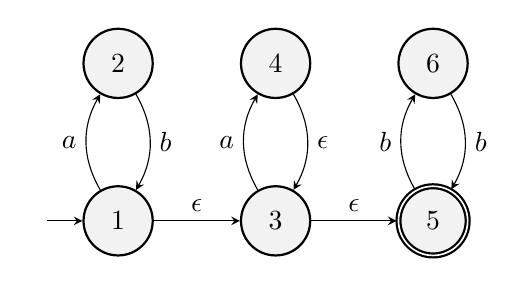
\begin{tikzpicture}
        \node[state,           ] (4) {$4$};
        \node[state, left  of=4] (2) {$2$};
        \node[state, right of=4] (6) {$6$};
        \node[state, initial, below of=2] (1) {$1$};
        \node[state, below of=4] (3) {$3$};
        \node[state, accepting, right of=3] (5) {$5$};
        
        \draw 
        (1) edge[above] node{$\epsilon$} (3)
        (3) edge[above] node{$\epsilon$} (5)
        
        (1) edge[bend left,left] node{$a$} (2)
        (2) edge[bend left,right] node{$b$} (1)
        
        (3) edge[bend left,left] node{$a$} (4)
        (4) edge[bend left,right] node{$\epsilon$} (3)
        
        (5) edge[bend left,left] node{$b$} (6)
        (6) edge[bend left,right] node{$b$} (5);
    \end{tikzpicture}
    \caption{A $\langle 2,3 \rangle$-flat automaton 
that recognizes $L\Def  (ab)^*(a)^*(bb)^*$}
    \label{fig: FA}
\end{figure}
} 
 %%%%%%%%%%%%%%%%%%%%%%%%%%%%%%%%%%%%%%%%
  %%%%%%%%%%%%%%%%%%%%%%%%%%%%%%%%%%%%%%%%
\hide{
\paragraph{Generic Flat Languages and Automata}
Fix $\alpha = \langle p,q \rangle$,
we define the \emph{generic $\alpha$-flat language} is the union of all $\alpha$-flat languages, denoted by $\mathbb{F}(\alpha)$.
Now, we try to define an automaton that recognizes all $\alpha$-flat languages,
i.e., collects all behaviors of $\alpha$-flat automata.

Intuitively, 
the generic automaton is obtained by introducing a new alphabet (
a multi-set with $p q$ copies of the original alphabet) and 
adding more transitions (labels),
the states and the overall framework remain unchanged. 
In details, a generic $\alpha$-flat automaton is still a finite state automaton over
$\Sigma(\alpha)\Def \{a(i)| (a\in \Sigma_\epsilon) \wedge i\in \mathbb{N}:1\le i \le pq\}\cup \{\epsilon\}$.
The states are still named from $1$ to $pq$, 
the initial state is $1$ and the accepting state is $(pq-p+1)$.
The transition relations for state $i$ are defined as 
\begin{itemize}
    \item if $i\  \text{mod}\  p = 1$ and $i\neq pq-p+1$, then 
    $(i,\epsilon,i+p)\in \Delta$
    and $\forall s\in \Sigma_{\epsilon}. (i, s(i) ,i+1) \in \Delta$;
    \item if $i\  \text{mod}\  p = 0$, 
    $\forall s \in \Sigma_{\epsilon}. (i,s(i), i-p+1) \in \Delta$;
    \item otherwise, $\forall s \in \Sigma_{\epsilon}. (i,s(i), i+1) \in \Delta$.
\end{itemize}

For $\Sigma = \{a,b\}$, an example of generic $\langle 2,3 \rangle$-flat automaton is shown in figure (\ref{fig: GFA}).

\begin{figure}[ht]
    \centering 
    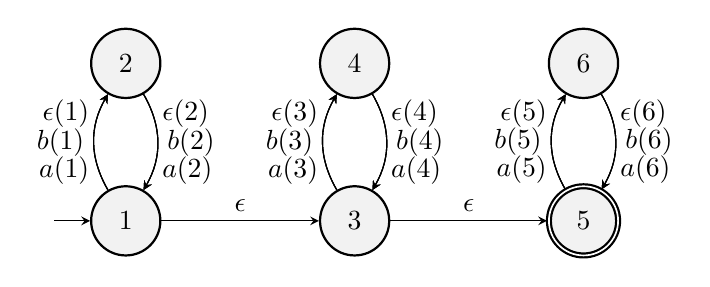
\begin{tikzpicture}
        \node[state,           ] (4) {$4$};
        \node[state, left  = 2cm of 4] (2) {$2$};
        \node[state, right = 2cm of 4] (6) {$6$};
        \node[state, initial, below of=2] (1) {$1$};
        \node[state, below of=4] (3) {$3$};
        \node[state, accepting, below of=6] (5) {$5$};
        
        \draw 
        (1) edge[above] node{$\epsilon$} (3)
        (3) edge[above] node{$\epsilon$} (5)
        
        (1) edge[bend left, pos =0.2 ,left] node{$a(1)$} (2)
        (1) edge[bend left, pos =0.5 ,left] node{$b(1)$} (2)
        (1) edge[bend left, pos =0.8 ,left] node{$\epsilon(1)$} (2)
        
        (2) edge[bend left, pos = 0.2 ,right] node{$\epsilon(2)$} (1)
        (2) edge[bend left, pos = 0.5 ,right] 
        node{$b(2)$} (1)
        (2) edge[bend left, pos = 0.8 ,right] 
        node{$a(2)$} (1)
        
        (3) edge[bend left, pos =0.2 ,left] node{$a(3)$} (4)
        (3) edge[bend left, pos =0.5 ,left] node{$b(3)$} (4)
        (3) edge[bend left, pos =0.8 ,left] node{$\epsilon(3)$} (4)
        
        (4) edge[bend left, pos = 0.2 ,right] node{$\epsilon(4)$} (3)
        (4) edge[bend left, pos = 0.5 ,right] 
        node{$b(4)$} (3)
        (4) edge[bend left, pos = 0.8 ,right] 
        node{$a(4)$} (3)
        
        (5) edge[bend left, pos =0.2 ,left] node{$a(5)$} (6)
        (5) edge[bend left, pos =0.5 ,left] node{$b(5)$} (6)
        (5) edge[bend left, pos =0.8 ,left] node{$\epsilon(5)$} (6)
        
        (6) edge[bend left, pos = 0.2 ,right] node{$\epsilon(6)$} (5)
        (6) edge[bend left, pos = 0.5 ,right] 
        node{$b(6)$} (5)
        (6) edge[bend left, pos = 0.8 ,right] 
        node{$a(6)$} (5);
    \end{tikzpicture}
    \caption{The generic $\langle 2,3 \rangle$-flat automaton}
    \label{fig: GFA}
\end{figure}
 

However,
the resulted automaton may accept languages that are not in $\mathbb{F}(\alpha)$,
because in different passes inside a loop, 
the automaton can choose different symbols between identical pairs. 
To avoid this problem,
we add a so-called purity condition on the accepting language of generic flat automata,
which is equivalent to intersecting the language of a generic flat automaton 
with a language that encodes the purity condition.

We say a string $w\in (\Sigma(\alpha))^*$ is pure if for all $i: 1\le i \le p q$,
and $a,b\in \Sigma$, 
$a\neq b \wedge \#w(a(i))>0$ implies $\#w(b(i))=0$.
Formally, the purity condition is defined by 
\begin{equation} \label{eq:purity}
 \bigwedge_{1\le i\le pq}\bigwedge_{a,b\in \Sigma, a\neq b} ({a(i)}^\#>0)\to ({b(i)}^\#=0)\, . 
\end{equation}

We denote the accepting language of the generic $\alpha$-flat automaton by $\mathbb{G}(\alpha)$.
Note that $\mathbb{G}(\alpha)$ is a language over $\Sigma_\alpha$,
but what we want is a language over $\Sigma$.
So we define a renaming function $R:\Sigma(\alpha)\mapsto \Sigma$ such that for all $a(i) \in \Sigma_\alpha, R(a(i))=a$,
and $R(\epsilon) = \epsilon$.
Define $\mathbb{G}'(\alpha) \, \Def \, \{R(w) \mid w\in \mathbb{G}(\alpha)\}$, 
for simplicity, we write
$\mathbb{G}'(\alpha)=R(\mathbb{G}(\alpha))$.

The important feature of generic flat autamata
is that every word $w\in \mathbb{G}(\alpha)$ is uniquely determined by its Parikh image $\mathbb{P}(w)$.
}



\section{Flattening string constraints with string-integer conversion}\label{sec:string-solving}

%!TEX root = paper.tex

In this section, we first define the class of string constraints with string-integer conversion, denoted by $\strint$. Then we define the extension of Presburger arithmetic with exponential functions, denoted by $\paexp$. Finally, we show how to flatten the string constraints in $\strint$ into the arithmetic constraints in $\paexp$.

\subsection{String constraints with string-integer conversion ($\strint$)}

In the sequel, we shall define $\strint$, the class of string constraints with the string-integer conversion function {\parseInt}.

The function  {\parseInt} takes a decimal string as the input and returns the integer represented by the string\footnote{The {\parseInt} function in scripting languages e.g. Javascript is more general in the sense that the base can be a number between 2 and 36. Although our approach works for arbitrary positive bases, we choose to focus on the base 10 in this paper, for readibility.}.
%Since we focus on the decidability,
%we define a binary version of {\parseInt},
%which takes a binary string and returns a decimal integer number.
For example,
${\parseInt}('0123') = {\parseInt}('123')=10^2+10*2+3 = 123$. 
Note here we use the quotation marks to delimit the strings, 
%Clearly,  our decision procedure given in this paper 
%can be adapted to string constraints with other string to number conversion function without substantial change. 
%Single quotation marks are used to distinguish a symbol like $'1'\in \Sigma$
%from a number $1_\mathbb{N}\in \mathbb{N}$ when needed.

Formally, the semantics of the $\parseInt$ function is defined as follows. 
%\begin{definition} 
Let $\Sigma_{\textit{num}}=\{0,1, \ldots, 9\}$. Then ${\parseInt}: \Sigma_{\textit{num}}^+ \mapsto \Nat$ is recursively defined by
    for every $w\in \Sigma_{\textit{num}}^+$,
    \begin{itemize}
%        \item if $|w|=0$, i.e., $w=\epsilon$,  ${\parseInt}(w)=0$;
        \item if $w={'i'}$ for $i \in \Sigma_{\textit{num}}$, then ${\parseInt}('i')=i$;
        \item for $w = w_1 {'i'}$ for $i \in \Sigma_{\textit{num}}$ with $|w_1| \ge 1$, 
        ${\parseInt}(w) = 10*{\parseInt}(w_1)+{\parseInt}({'i'})$.
    \end{itemize} 
%\end{definition}
Note that $\parseInt$ is undefined with $\varepsilon$ as the input.


In $\strint$, there are two types of variables, namely, the string variables $\svarx,\svary,\ldots \in \svars$ and the integer variables $\ivarx,\ivary,\ldots \in \ivars$.
%
A $\strint$ formula $\varphi$ is defined by the following rules, where $\len(\sterm)$ denotes the length of a string $\sterm$.
\[
\begin{array}{l c l}
\sterm & \Def & a \mid \svarx \mid \sterm \concat \sterm, \\
\iterm & \Def & n \mid \ivarx \mid \len(\sterm) \mid \parseInt(\sterm) \mid \iterm + \iterm \mid \iterm - \iterm,\\
\varphi & \Def & \sterm = \sterm \mid x \in \Aut \mid \iterm\ \op\ \iterm \mid \varphi \wedge \varphi \mid \varphi \vee \varphi \mid \neg \varphi,
\end{array}
\]
where $a \in (\Sigma_{\textit{num}})_\varepsilon$, $n \in \Nat$, $\Aut$ is an FA, and $\op \in \{=, < , >, \le, \ge\}$. Let us call $\sterm$ as string terms, $\iterm$ as integer terms, $\sterm = \sterm$ as string equality constraints, $x \in \Aut$ as regular constraints, $\iterm \op\ \iterm$ as arithmetic constraints. 
Let  $\svar(\varphi)$ and $\ivar(\varphi)$ denote the set of string variables and integer variables respectively occurring in $\varphi$.


%%%%%%%%%%%%%%%%%%%%%%%%%%%%%%%%
%%%%%%%%%%%%%%%%%%%%%%%%%%%%%%%%
\hide{
\paragraph{String Terms}
Given a finite alphabet $\Sigma$ and 
a finite set $X$ of string variables over $\Sigma^*$,
we define the set of terms $\textit{Terms}(\Sigma,X)$ 
to be the smallest set satisfying
\begin{itemize}
    \item[1] $\Sigma\cup \{\epsilon\} \cup X \subseteq \textit{Terms}(\Sigma,X)$;
    \item[2] if $t_1,t_2\in \textit{Terms}(\Sigma,X)$, then $t_1 \cdot t_2 \in \textit{Terms}(\Sigma,X)$.
\end{itemize} 

We extend $I_X$ to $\textit{Terms}(\Sigma,X)$ by letting $I_X(\epsilon)=\epsilon$, 
for $a\in \Sigma, I_X(a)=a$,
and $I_X(t_1\cdot t_2)= I_X(t_1)\cdot I_X(t_2)$.

\paragraph{String Constraints} \label{par: string constraints}
Given a constraint $\phi$ and an interpretation $I$,
$I\models \phi$ denotes that $I$ satisfies $\phi$,
and $I$ is called a \emph{model} of $\phi$.
We use $\lVert \phi\rVert$ to denote the set of all models of $\phi$.

We define the following three forms of atomic string constraints:
\begin{itemize}
\item An equality constraint $\phi_e$ is of the form 
$t_1 = t_2$, where $t_1,t_2\in \textit{Terms}(\Sigma,X)$.
We define $\lVert \phi_e \rVert = \{I\mid I(t_1)=I(t_2)\}$.
Inequality constraints can be defined analogously.

\item A regular constraint $\phi_r$ is of the form 
$x\in L(\mathcal{A})$,
where $x\in \mathbb{X}$ and $\mathcal{A}$ is a finite state automaton.
We define $\lVert \phi_r \rVert = \{I\mid I(x)\in L(\mathcal{A})\}$.

\item A length constraint $\phi_l$ is a linear constraint over 
$Z \cup \{|x| \mid x\in X\}$, %the values of $|x|$ for all $x\in X$,
where $|\cdot |$ is the length function.
We define $\lVert \phi_l \rVert = \{I \mid I\models \phi_l \}$.
\end{itemize}
}
%%%%%%%%%%%%%%%%%%%%%%%%%%%%%%%%
%%%%%%%%%%%%%%%%%%%%%%%%%%%%%%%%

The $\strint$ formulas are interpreted on $I=(I_s, I_i)$ where $I_s$ is a partial function from $\svars$ (the set of string variables) to $\Sigma^*$ and $I_i$ is a partial function from $\ivars$ (the set of integer variables) to $\Nat$. Moreover, it is required that the domains of $I_s, I_i$ are finite. Given $I = (I_s, I_i)$, the interpretations of string terms, integer terms, as well as the formulas $\varphi$ under $I$ are easy to comprehend, thus omitted to avoid tediousness. For $\varphi \in \strint$ and $I = (I_s, I_i)$, $I$ satisfies $\varphi$ if the interpretation of $\varphi$ under $I$ is $\ltrue$.
Let us use $\lVert \varphi \rVert$ to denote the set of $I = (I_s, I_i)$ satisfying $\varphi$.

\begin{example}
some example for $\strint$ here
\end{example}

%As usual, an interpretation $I$ is a mapping from the set of variables $X\cup Z$ to the respective domain, 
%essentially a pair of two mappings 
%$I_X$ and $I_Z$, i.e., $I= (I_X, I_Z)$,  
%where $I_X$ is a mapping in $X \mapsto \Sigma^*$ and $I_Z$ is a mapping in $Z \mapsto \mathbb{N}$.

The satisfiability problem of $\strint$ is to decide for a given constraint $\varphi \in \strint$,
whether $\lVert  \varphi \rVert \neq \emptyset$.
%if not, to compute an interpretation $I$ that satisfies $\Psi$.

\subsection{An Extension of Presburger Arithmetic with Exponential Functions ($\paexp$)}


%%%%%%%%%%%%%%%%%%%%%%%%%%%%%
%%%%%%%%%%%%%%%%%%%%%%%%%%%%%
\hide{
For a first order theory $T$,
we say theory $T$ admits quantifier elimination (QE) if for any formula in $T$, 
there is a quantifier-free formula equivalent to it.
It is well-known that if a theory admits QE, 
then it is a decidable theory.

The formal definition of PA is given in section \ref{PA}.
Here we add the ordering predicate $\le$ into the signature,
which can be defined by $x \le y\, \Def \, \exists z. x+z=y$.
However, the theory PA so far does not admit QE, 
for example, consider the formula $\exists x.x = y + y$. 
We augment the theory with countable unary divisible predicates
$n|x$, where $n\in \mathbb{N}$, 
$n|x$ is true if and only if $x\ \text{mod}\ n=0$ holds.
This structure of PA that admits QE is denoted by $(\mathbb{N},+)$.
}
%%%%%%%%%%%%%%%%%%%%%%%%%%%%%
%%%%%%%%%%%%%%%%%%%%%%%%%%%%%

{\paexp} extends Presburger arithmetic with the exponential function $10^x$ as well as the (partial) functions $\ell_{10}(\ivarx)$ and $\lambda_{10}(\ivarx)$ (cf. \cite{Point86}). The functions $\ell_{10}(\ivarx)$ and $\lambda_{10}(\ivarx)$ are inductively defined as follows.
\begin{itemize}
\item The (partial) function $\ell_{10}(\ivarx)$ is inductively defined as follows: For $n \ge 1$, $\ell_{10}(n) = m$ iff $10^m \le n < 10^{m+1}$. \wuhao{For $n \le 0$, we define $\ell_{10}(n)=0$}

%(Note that $\ell_{10}(0)$ is undefined.) 
%
\item The (partial) function $\lambda_{10}(\ivarx)$ can be defined by $\ell_{10}(\ivarx)$: For $n \ge 1$, $\lambda_{10}(n) = 10^{\ell_{10}(n)}$. (Intuitively, $\lambda_{10}(\ivarx)$ is the maximum power of 10 that is no greater than $\ivarx$.)
\end{itemize}

The syntax of {\paexp} is obtained from that of {\pa} by adding $10^\iterm$, $\ell_{10}(\iterm)$ and $\lambda_{10}(\iterm)$ to the definition of integer terms. Specifically, {\paexp} formulas are defined by the rules,
%
 $$
 \begin{array}{ l c l}
 \iterm &\Def& c \mid \ivarx \mid \iterm + \iterm \mid \iterm - \iterm \mid 10^\iterm \mid \ell_{10}(\iterm) \mid \lambda_{10}(\iterm), \\
 \phi &\Def & \iterm \ \op\ \iterm \mid c | \iterm \mid \phi \wedge \phi \mid \phi \vee \phi \mid \neg \phi \mid \exists \ivarx.\ \phi \mid \forall \ivarx.\ \phi.
 \end{array}
 $$
 The semantics of {\paexp} are defined similarly as {\pa}.

\begin{example}
Some example of  {\paexp} here.
\end{example} 
 
%Moreover, we introduce an abbreviation $\lambda_{10}(\ivarx) \equiv 2^{\ell_{10}(\ivarx)}$.
From the definition of $\lambda_{10}(\ivarx)$, we know that for all $n \ge 1$, $\lambda_{10}(n) \le n \le 10\lambda_{10}(n)-1$ holds.


%%%%%%%%%%%%%%%%%%%%%%%%%%%%%%%%%%%%
%%%%%%%%%%%%%%%%%%%%%%%%%%%%%%%%%%%%
\hide{
\begin{definition}
    Let $\mathcal{L}=\{0,1,+,\le,n \, |x(n\in \mathbb{N}),2^x,l_2(x)\}$, 
     $(\mathbb{N},+,2^x)$ be a $\mathcal{L}$-theory that has domain $\mathbb{N}$, where 
    \begin{itemize}
        \item  $2^x$ is interpreted to the exponential function of $2$ over $\mathbb{N}$; 
        \item interpretations of $0,1,+,\le,=$ are consistent with PA;
        \item for $n\ge 1$,$n|x$ holds iff $\exists y.x=ny$;
        \item $2^0=1$, for $n \ge 1, 2^n = 2^{n-1}+2^{n-1}$;
        We further assume that if $m,n\in \mathbb{N}, m\le n$, 
        then $2^{m-n} = 1$
        \item $l_2(0)=0$; for $n \ge 1,l_2(n) = y$ iff $2^y \le n < 2^{y+1}$;  $l_2(m-n) = 0$
        if $m,n\in \mathbb{N}$ and $m\le n$. 
    \end{itemize}
\end{definition}

$\lambda_2(x) = 2^{l_2(x)}$ can be defined by $l_2(x)$,
intuitively, $\lambda_2(x)$ means the maximal power of 2 that is not larger than $x$.
Then we have $\lambda_2(x) \le x \le 2\lambda_2(x)-1$,
which will be useful in our proof. 
}
%%%%%%%%%%%%%%%%%%%%%%%%%%%%%%%%%%%%
%%%%%%%%%%%%%%%%%%%%%%%%%%%%%%%%%%%%

\subsection{Flattening $\strint$ into $\paexp$}

We first recall the flattening approach for string constraints in \cite{Parosh:20:PLDI}, then show how to extend it to deal with the {\parseInt} function.

A \emph{flat domain restriction} for a string constraint $\varphi$ is a function $\flatfun_\varphi$ that maps each string variable $\svarx \in \svar(\varphi)$ to a flat language $(w_{\svarx,1})^* \cdots (w_{\svarx, k_\svarx})^*$, where $w_{\svarx, i} \in \Sigma_{\textit{num}}^+$ for every $i \in [k_\svarx]$. 
%
The flattened semantics of $\phi \in \strint$ is defined as $\llbracket \varphi \rrbracket_{\flatfun_\varphi} = \{(I_s, I_i) \in \llbracket \varphi  \rrbracket \mid \forall \svarx \in \svar(\varphi).\ I_s(x) \in  \flatfun_\varphi(\svarx)\}$.  

The flattening of $\varphi \in \strint$ under a flat domain restriction $\flatfun_\varphi$ is a {\paexp} formula, denoted by $\flatten_{\flatfun_\varphi}(\varphi)$, that encodes its flattened semantics.
%
More concretely, $\flatten_{\flatfun_\varphi}(\varphi)$ is a formula over the integer variables $\ivar(\varphi)$,  and Parikh variables $\pvar_{\flatfun_\varphi}(\varphi) = \bigcup_{\svarx \in \svar(\varphi)} \pvar_{\flatfun_\varphi}(\svarx)$, where $\pvar_{\flatfun_\varphi}(\svarx) = \{\#_{\svarx,i} \mid i \in [k_\svarx]\}$, called \emph{flattening variables}, plus some other auxiliary variables, such that 
%
$$\llbracket \phi \rrbracket_\kell =\decode_{\flatfun_\varphi}(\llbracket \flatten_{\flatfun_\varphi}(\varphi) \rrbracket |_{\ivar(\phi) \cup \pvar_{\flatfun_\varphi}(\varphi)})$$
%
The decoding function above decodes an interpretation of integer and flattening variables $I_e: \ivar(\varphi) \cup \pvar_{\flatfun_\varphi}(\varphi) \rightarrow \Nat$ as a set $\decode_{\flatfun_\varphi}(I_e)$ of interpretations of the $\varphi$'s integer and string variables $(I_s, I_i)$ with $I_s: \svar(\varphi) \rightarrow \Sigma^*$ and $I_i: \ivar(\phi) \rightarrow \Nat$ such that 
\begin{itemize}
\item  
for every $ \svarx \in \svar(\varphi)$, $I_s(\svarx) = w_{\svarx,1}^{I_e(\#_{\svarx,1})} \ldots  w_{\svarx,k_\svarx}^{I_e(\#_{\svarx,k_\svarx})}$, 
%
\item for every $ \ivarx \in \ivar(\varphi)$, $I_i(\ivarx) = I_e(\ivarx)$.
\end{itemize}

The formula $\flatten_{\flatfun_\varphi}(\varphi)$ is constructed inductively by following the structure of $\varphi$: $\flatten_{\flatfun_\varphi}(\varphi_1\ \mathfrak{o}\ \varphi_2) = \flatten_{\flatfun_\varphi}(\varphi_1) \ \mathfrak{o}\  \flatten_{\flatfun_\varphi}(\varphi_2)$, where $\mathfrak{o} \in \{\wedge, \vee\}$, and $\flatten_{\flatfun_\varphi}(\neg \varphi_1) = \neg \flatten_{\flatfun_\varphi}(\varphi_1)$. Therefore, it is sufficient to show how to construct $\flatten_{\flatfun_\varphi}(\varphi)$ for atomic constraints $\varphi$. 
In the sequel, we will show how to construct $\flatten_{\flatfun_\varphi}(\iterm_1 \op \iterm_2)$ where $\parseInt(\sterm)$ may occur in $\iterm_1$ or $\iterm_2$. The construction of $\flatten_{\flatfun_\varphi}(\varphi)$ for the other atomic constraints is essentially the same as that in \cite{Parosh:20:PLDI} and thus omitted. 


%%%%%%%%%%%%%%%%%%%%%%%%%%%%%%%%%%%%%%%%%%%%%%%%%
%%%%%%%%%%%%%%%%%%%%%%%%%%%%%%%%%%%%%%%%%%%%%%%%%
\hide{
The flattening technique was first introduced 
in \cite{Abdulla 2017}.
Fix an alphabet $\Sigma$ and an abstraction parameter $\alpha$, 
for a given atomic string constraint $\phi$, 
flattening $\phi$ with parameter $\alpha$ 
results in a new string constraint $\phi_\alpha$,
such that 
$R(\lVert \phi_\alpha \rVert) = \lVert \phi \rVert \cap \{I \mid \forall x\in X, I(x)\in \mathbb{G}'(\alpha)\}$,
where $R$ is the renaming function with its domain extended to interpretations in the normal manner.
Intuitively, it restricts $\phi$ to interpret 
string variables over $\mathbb{G}'(\alpha)$.

\cite{Abdulla 2017} discussed the flattening of basic 
string constraints including equality, integer, (regular) grammar and transducer constraints. 
For an atomic string constraint $\phi$,
the flattening $\phi_\alpha$ is still an atomic string constraint 
and is Parikh definable,
so its Parikh image can be expressed by a quantifier free PA formula.
Together with the purity condition,
we obtain an existential quantified PA formula $\rho$.
$\rho$ will be sent to a SMT solver,
if the solver returns an solution $\theta$,
then we can construct an interpretation for $\phi_\alpha$ from $\theta$,
otherwise it means $\phi$ is unsatistiable when 
string variables are interpreted  to $\alpha$-flat languages.

Take a regular constraint $\phi = x\in L(A)$ for example,
the flattening of $\phi$ resutls in a new finite state automaton $A'$ over $\Sigma(\alpha)$,
which encodes running $A$ ``in parallel" 
with the generic $\alpha$-flat automaton.
Let $\rho_1$ be the formula describing the Parikh image of $A'$,
which is a formula over variable sets $\Sigma(\alpha)^\#$.
Let $\rho_2$ be the purity condition \eqref{eq:purity}.
Then we obtain the PA formula $\exists (\Sigma(\alpha))^\#. \rho_1 \wedge \rho_2$.
In order to distinguish between different string variables,
we may replace $a(i)^\# \in \Sigma(\alpha)^\#$ by $(x,a(i))^\#$.

Since the structure of a flat automaton is decided 
by its abstraction parameter $\alpha$, 
a Counter-Example Guided Abstraction 
Refinement (CEGAR) framework is designed, which contains both an under- and an 
over-approximation module, to search the possible values of $\alpha$.
The termination for the overall algorithm is not guaranteed.


The string-number conversion functions are commonly used functions
in most of programming languages,
for example,
\verb+parseInt()+ in Java and \verb+Int()+ in Python.
The functions usually take two parameters, 
a string over the agreed alphabet $\Sigma$
and an optional parameter denotes the radix.
They parse the string according to the rules indicated by the radix,
and return an integer denoted by the string.

From the view of string constraints,
string-number conversion functions give rise to a new form of string constraints
and are more expressive than length constraints.
So we consider extending string constraints with 
{\parseInt} function. 
As the general problem of string constraints is undecidable,
we still adopt the idea of flattening, 
i.e., variables are restricted to (generic) flat languages.
This problem has been investigated in \cite{POPL20},
which defined a special form of flat restriction (straight-line PFA) and 
proposed a heuristic search method.

In this section, 
we describe the problem of interest first, and then 
present an reduction from the problem of solving flat string constraints with {\parseInt} function
to the decidability problem of Presburger Arithmetic with exponential functions.
Hence, we identify a decidable subset of string constraints, which is the largest one with decidability so far to the best of our knowledge.
}
%%%%%%%%%%%%%%%%%%%%%%%%%%%%%%%%%%%%%%%%%%%%%%%%%
%%%%%%%%%%%%%%%%%%%%%%%%%%%%%%%%%%%%%%%%%%%%%%%%%

Before presenting the construction of $\flatten_{\flatfun_\varphi}(\iterm_1 \op \iterm_2)$, for every $\svarx \in \svar(\varphi)$, we define $\flatten_{\flatfun_\varphi}(\parseInt(\svarx)) = \iterm_{\svarx,1}$  such that $(\iterm_{\svarx, i})_{i \in [k_\svarx]}$ and $(\ell_{\svarx, i})_{i \in [k_\svarx]}$ are inductively defined as follows: 
\begin{itemize}
\item for $i = k_\svarx$, 
$$\iterm_{\svarx, i} = \frac{\parseInt(w_{\svarx, k_\svarx}) (10^{|w_{\svarx,k_\svarx}| \#_{\svarx, k_\svarx} } -1 )}{(10^{|w_{\svarx, k_\svarx}|} -1 )}$$ 
and $\ell_{\svarx, i} = |w_{\svarx,k_\svarx}| \#_{\svarx, k_\svarx}$,
%
\item for $i \in [k_\svarx-1]$, 
%
$$\iterm_{\svarx, i} =  \frac{\parseInt(w_{\svarx, i}) (10^{|w_{\svarx, i} | \#_{\svarx, i} } -1 ) 10^{\ell_{\svarx, i+1}}} {(10^{|w_{\svarx, i}|} -1 )} + \iterm_{\svarx, i+1}$$
%
and $\ell_{\svarx, i} = |w_{\svarx, i} | \#_{\svarx, i} + \ell_{\svarx, i+1}$.
\end{itemize}

Then $\flatten_{\flatfun_\varphi}(\iterm_1 \op \iterm_2)$ is obtained from $\iterm_1 \op \iterm_2$ by the following procedure.
\begin{enumerate}
\item Replace each integer term $\len(t)$ such that $t = \alpha_1 \ldots \alpha_m$ with $\alpha_i \in \Sigma_{\textit{num}} \cup \svar(\varphi)$ for every $i \in [m]$, by 
 $\sum \limits_{i \in [m]} \theta_i$, where for every $i \in [m]$, $\theta_i = 1$ if $\alpha_i \in \Sigma_{\textit{num}}$ and $ \theta_i = \sum \limits_{j \in [k_{\alpha_i}]} |w_{\alpha_i, j} | \#_{\alpha_i, j}$ otherwise.
%
\item  Replace each integer term $\parseInt(\sterm)$ such that $t = \alpha_1 \ldots \alpha_m$ with $\alpha_i \in \Sigma_{\textit{num}} \cup \svar(\varphi)$ for every $i \in [m]$, by $\iterm_{\parseInt(\sterm)}$, where $\iterm_{\parseInt(\sterm)} = \iterm_{t,1}$ such that $(\iterm_{t,i})_{i \in [m]}$ and $(\ell_{t, i})_{i \in [m]}$ are inductively defined as follows: 
\begin{itemize}
\item if $\alpha_m \in \Sigma_{\textit{num}}$, then $\iterm_{t, m} = \alpha_m$ and $\ell_{t, m} = 1$, otherwise, $\iterm_{t, m} = \flatten_{\flatfun_\varphi}(\parseInt(\alpha_m))$ and $\ell_{t, m} = \sum \limits_{j \in [k_{\alpha_m}]} |w_{\alpha_m, j}| \#_{\alpha_m, j}$,
%
\item for $i \in [m-1]$, if $\alpha_i \in \Sigma_{\textit{num}}$, then $\iterm_{t, i} = \alpha_i 10^{\ell_{t, i+1}} + \iterm_{t, i+1}$ and $\ell_{t, i} = \ell_{t, i+1}+1$, otherwise, $\iterm_{t, i} = 
\flatten_{\flatfun_\varphi}(\parseInt(\alpha_i))10^{\ell_{t, i+1}}  + \iterm_{t, i+1}$ and $\ell_{t, i} = \ell_{t, i+1} + \sum \limits_{j \in [k_{\alpha_i}]} |w_{\alpha_i, j}| \#_{\alpha_i, j}$.
\end{itemize}
%
\item Let $\iterm'_1 \op \iterm'_2$ be the formula resulting from the aforementioned replacements. (Note that strictly speaking, $\iterm'_1 \op \iterm'_2$ is not a $\paexp$ formula since it contains divisions.) Let $N$ be the least common multiplier of the denominators of $\iterm'_1$ and $\iterm'_2$.  Then $\flatten_{\flatfun_\varphi}(\iterm_1 \op \iterm_2)$ is obtained by multiplying the both sides of $\iterm'_1 \op \iterm'_2$ with $N$,  so that the division operator disappears. 
\end{enumerate}

\begin{example}
Suppose $\parseInt(\svarx) = 2\ivarx$ is an atomic constraint and $\flatfun_\varphi(\svarx) = 1^*2^*$. Then 
\[
\small
\begin{array}{l l}
& \flatten_{\flatfun_\varphi}(\parseInt(\svarx)  =  2\ivarx)  \\
\Def & 1 \frac{10^{\#_{\svarx,1}}-1}{10-1}10^{\#_{\svarx,2}}  + 2 \frac{10^{\#_{\svarx,2}}-1}{10-1} = 2\ivarx   \\
\equiv & 10^{\#_{\svarx,1}+\#_{\svarx,2}} - 10^{\#_{\svarx,2}}  + 2 (10^{2\#_{\svarx,2}}-1) = 18\ivarx \\
\equiv & 10^{\#_{\svarx,1}+\#_{\svarx,2}} +  10^{\#_{\svarx,2}} = 18\ivarx + 2.
\end{array}
\]
%Take $n={\parseInt}((11)^a(10)^b)$ for example.
%\begin{align}
%    n=& {\parseInt}((11)^a)\cdot 2^{2b} + {\parseInt}((10)^b) \notag \\
%    =& {\parseInt}(11)\cdot \frac{2^{2a}-1}{2^2-1}\cdot 2^{2b} + 
%    {\parseInt}(10) \cdot \frac{2^{2b}-1}{2^2-1} \notag 
%\end{align}
\end{example}



%%%%%%%%%%%%%%%%%%%%%%%%%%%%%%%%%%%%%%%%%%%
%%%%%%%%%%%%%%%%%%%%%%%%%%%%%%%%%%%%%%%%%%%
\hide{
Now, we introduce a new form of atomic string constraints: 
a {\parseInt} constraint $\phi$ is of the form 
$n \sim {\parseInt}(t)$,
where $n$ is an integer term, $\sim \in \{\le,<,=,>,\ge\}$ and $t\in \textit{Terms}(\Sigma_{\textit{num}},X)$ is a string term.
$\lVert \phi\rVert \Def  \{I \mid I(n)\sim {\parseInt}(I(t))\}$.

In what follows, we only  consider the problem in the case when $t=x$ and $x$ is restricted to (generic) flat languages. 
%If $t$ is not a single variable, 
For the general case $t\in \textit{Terms}(\Sigma_{\textit{num}},X)$, 
it can be reduced to this special case by induction on the structure of $t$. 
%we can reduce the problem by separating $t$ (corresponding to the $|w|>2$ case in definition).

Given an $\alpha$-flat language $L$,
we assume $\alpha=\langle p,q \rangle$ and $L=(w_1)^*...(w_q)^*$,
where $p,q$ and $w_i(1\le i \le q) $ are known.
We further assume that $x = (w_1)^{\beta_1} ... (w_q)^{\beta_q}$,
then we have
\begin{align}
    &{\parseInt}(x) \notag \\
    =&{\parseInt}((w_1)^{\beta_1} ... (w_q)^{\beta_q}) \notag \\
    =&{\parseInt}((w_1)^{\beta_1} ... (w_{q-1})^{\beta_{q-1}})\cdot 2^{\beta_q |w_q|}
    + {\parseInt}((w_q)^{\beta_q}) \label{parse}
\end{align}
(\ref{parse}) is a recursive expression.
So we only need to deal with the basic case ${\parseInt}((w_q)^{\beta_q})$, 
where $w_q \neq \epsilon$
\begin{align}
    {\parseInt}((w_q)^{\beta_q}) &= \sum_{i=0}^{\beta_q-1} {\parseInt}(w_q)\cdot 2^{|w_q|\cdot i}  \notag \\
    &={\parseInt}(w_q)\frac{2^{|w_q|\cdot \beta_q}-1}{2^{|w_q|}-1}
    \label{parseInt-basic}
\end{align}
In (\ref{parseInt-basic}), since $w_q$ and $|w_q|$ are known, 
they can be regarded as constants.
The only unknown variable is $\beta_q$.

Combine (\ref{parse}) and (\ref{parseInt-basic}),
the constraint $n={\parseInt}(x)$ can be expressed by an arithmetic expression with 
$n$ and $(\beta_1,...,\beta_q)$,
inevitably with exponential components.

Observe the form of the above equation,
$a,b,n$ are integer variables and either occur in 
an exponential term or a linear term.
This is always the case,
so the problem can be reduced to 
the decidability of PA with exponential function.

When $x$ of {\parseInt} constraints is restricted to the
generic $\alpha$-flat language ($\alpha$ is fixed),
the (\ref{parse}) and (\ref{parseInt-basic}) still hold 
but $w_i(1\le i\le q)$ is known.
However,
by definition,
the generic $\alpha$-flat language is the finite union of all $\alpha$-flat languages,
so we can enumerate all possible values for $w_i$.
In this way,
the problem can still be reduced to the decidability of PA with exponential function ($\paexp$), i.e.,
\begin{theorem} \label{thm:string-parInt}
If {$\paexp$} is decidable, then the satisfiability (validity) of string constraints with {\parseInt} in which all string variables 
are ranged over flat strings is decidable. 
\end{theorem}
}
%%%%%%%%%%%%%%%%%%%%%%%%%%%%%%%%%%%%%%%%%%%
%%%%%%%%%%%%%%%%%%%%%%%%%%%%%%%%%%%%%%%%%%%





\section{Decision procedure for $\paexp$}

%!TEX root = paper.tex

Semënov first proved that  {\paexp} admits quantifier elimination in \cite{Semenov84}, thus its satisfiability problem is decidable. However, Semënov did not give a concrete quantifier elimination procedure. Remedying this, Point proposed a quantifier elimination procedure for {\paexp} in \cite{Point86}. 

In this section, we describe how Point's quantifier elimination procedure works. 
%
\begin{theorem}[\cite{Point86}]
\label{thm-paexp}
{\paexp} admits quantifier elimination. 
\end{theorem}
%
Compared to \cite{Point86}, the presentation here is more accessible to computer science researchers. Moreover, the procedure presented here slightly improves Point's procedure, in the following two aspects: 1) DNF (disjunctive normal form) was required in Point's procedure, which is not required here, 2) in Point's procedure, the divisibility constraints produced by the elimination of linear occurrences of a variable should be converted to equality constraints (by introducing fresh variables) before the elimination of exponential occurrences of some other variable, which is unnecessary here, since the divisibility constraints are directly dealt with in the elimination of exponential occurrences of variables. 
%

However, in the next section we analyse the complexity of Point's procedure to be 3-EXPSPACE, which  is quite expensive and a faithful implementation would not scale\footnote{We did implement Point's algorithm and discovered that the implementation could only solve formulas of very small size.}.
So in Section~\ref{sec-opt}, we will propose various optimizations to Point's algorithm, aiming at an efficient implementation. 

\smallskip

As $\forall \ivarx. \ \varphi$ is equivalent to $\neg \exists \ivarx. \ \neg \varphi$,  thus in the sequel, we only need to  show that every $\paexp$ formula $\exists \ivarx.\ \varphi \in \paexp$, where $\varphi$ is quantifier-free, can be transformed into an equivalent quantifier-free formula $\varphi' \in \paexp$.

% when the quantifier elimination problem of $\paexp$  can be easily reduced to the above special case. 

% such that $\free(\varphi') = \free(\varphi) \setminus \{\ivarx\}$. 
%From this, we can easily derive that every {\paexp} formula $\varphi$ can be transformed effectively into an equivalent quantifier-free Presburger arithmetic formula $\varphi'$.

Before a formal description of the quantifier elimination procedure, let us use a simple example to illustrate the main idea and give an overview of the procedure.

\vspace{-4mm}

%\begin{example}
\subsection{An overview of the quantifier elimination procedure}
Consider $\varphi \Def \exists \ivarx_2.\ 10^{\ivarx_1 + \ivarx_2} - 10^{\ivarx_2} \le \ivary + 1001$. 

At first, we \emph{normalize} $\varphi$ by introducing a fresh variable $\ivarx_3$ for $\ivarx_1 + \ivarx_2$ and get the formula 
$$\varphi_1 \Def \exists \ivarx_3 \exists \ivarx_2.\ 10^{\ivarx_3} - 10^{\ivarx_2} \le \ivary + 1001 \wedge \ivarx_3 = \ivarx_1 + \ivarx_2.$$

Then, we enumerate different \emph{orders} of the quantified variables, i.e. $\ivarx_2$ and $\ivarx_3$. Since $\ivarx_3 = \ivarx_1 + \ivarx_2$, there is only one possible order, that is, $\ivarx_3 \ge \ivarx_2$.

Next, we illustrate how to eliminate the quantifier $\exists \ivarx_3$, assuming $\ivarx_3 \ge \ivarx_2$. The elimination of $\exists \ivarx_2$ is similar and simpler, thus omitted.

The elimination of $\exists \ivarx_3$ consists of two steps, namely, eliminating the exponential occurrences of $\ivarx_3$ first, and the linear occurrences next.

The main idea of the elimination of the exponential occurrences of $\ivarx_3$ is to observe that if $\ivarx_3 \ge \ell_{10}(\ivary+1001)+2$ and $\ivarx_3 \ge \ivarx_2 + 3$, then $10^{\ivarx_3} - 10^{\ivarx_2}$ is dominated by $10^{\ivarx_3}$, that is, $10^{\ivarx_3} - 10^{\ivarx_2} \ge 10^{\ivarx_3} - 10^{\ivarx_3 - 3} = (1-10^{-3}) 10^{\ivarx_3} \ge 10^{\ell_{10}(\ivary+1001)+1} = 10\lambda_{10}(\ivary+1001) > \ivary+1001$ (see Lemma~\ref{lem:exp-ineq} for the choice of the constants $2$ and $3$ in $\ivarx_3 \ge \ell_{10}(\ivary+1001)+2$ and $\ivarx_3 \ge \ivarx_2 + 3$.). 
Therefore, a necessary condition for $10^{\ivarx_3} - 10^{\ivarx_2} \le \ivary + 1001$ is that either $\ivarx_3 \le \ell_{10}(\ivary+1001)+1$ or $\ivarx_3 \le \ivarx_2 + 2$ holds.  

%\yfc{why $+2$ and $+3$ in $\ivarx_3 \ge \ell_{10}(\ivary+1001)+2$ and $\ivarx_3 \ge \ivarx_2 + 3$?}
\begin{itemize}
\item If $\ivarx_3 \le \ell_{10}(\ivary+1001)+1$, then we distinguish between whether $\ivarx_3 \le \ell_{10}(\ivary+1001)$ or  $\ivarx_3 = \ell_{10}(\ivary+1001)+1$. 
\begin{itemize}
\item If $\ivarx_3 \le \ell_{10}(\ivary+1001)$, then $10^{\ivarx_3} - 10^{\ivarx_2} \le 10^{\ell_{10}(\ivary+1001)} = \lambda_{10}(\ivary+1001) \le \ivary + 1001$. In this case, $10^{\ivarx_3} - 10^{\ivarx_2} \le \ivary + 1001 \wedge \ivarx_3 = \ivarx_1 + \ivarx_2$ can simplified into $\ltrue$.
%
\item If $\ivarx_3 = \ell_{10}(\ivary+1001)+1$, then $10^{\ivarx_3} - 10^{\ivarx_2} \le \ivary + 1001$ can be turned into $10^{\ell_{10}(\ivary+1001)+1} - 10^{\ivarx_2} \le \ivary + 1001 \equiv 10 \lambda_{10}(\ivary+1001) - 10^{\ivarx_2} \le \ivary + 1001 $.
\end{itemize} 
%
\item If $\ivarx_3 \le \ivarx_2 + 2$, then $\ivarx_3 = \ivarx_2 + j$ for $j \in \{0,1,2\}$. Thus $10^{\ivarx_3} - 10^{\ivarx_2} \le \ivary + 1001$ can be transformed to $\bigvee \limits_{j \in \{0,1,2\}} 10^{\ivarx_2 + j} - 10^{\ivarx_2} \le \ivary + 1001$.
\end{itemize}

To summarize, $\varphi_1$ is transformed into 
\[
\small
\begin{array}{l}
\varphi_2 \Def \exists \ivarx_3 \exists \ivarx_2. \\
\begin{array}{l}
\vspace{2mm}
\left(
\begin{array}{l}
\ivarx_3 \le \ell_{10}(\ivary+1001)\ \vee \\
\left(
\begin{array}{l}
\ivarx_3 = \ell_{10}(\ivary+1001)+1\ \wedge \\
10 \lambda_{10}(\ivary+1001) - 10^{\ivarx_2} \le \ivary + 1001 
\end{array}
\right) \vee \\
%
 \bigvee \limits_{j \in \{0,1,2\}}  \left(\ivarx_3 = \ivarx_2 +j \wedge 10^{\ivarx_2 + j} - 10^{\ivarx_2} \le \ivary + 1001\right)
\end{array}
\right) 
\wedge \\
 \ivarx_3 = \ivarx_1 + \ivarx_2.
 \end{array}
\end{array}
\]
Note that $\varphi_2$ contains \emph{only linear} occurrences of $\ivarx_3$.

Finally, we can eliminate the linear occurrences of $\ivarx_3$, thus the quantifier $\exists \ivarx_3$, by applying the quantifier elimination algorithm of {\pa}, e.g. Cooper's algorithm in \cite{Cooper72}. The elimination of $\ivarx_3$ in $\varphi_2$ here is simple, with $\ivarx_3$ replaced by $\ivarx_1 + \ivarx_2$. 

In the remainder of this section, we are going to describe the aforementioned steps of the decision procedures: Normalization, the enumeration of the variable orders, 
the elimination of the exponential occurrences of variables. The elimination of the  linear occurrences of variables is essentially the quantifier elimination of the {\pa} and omitted.

Let us assume that $\varphi \Def \exists \ivarx.\ \varphi'(\ivarx, \vec{\ivary})$, where $\varphi'$ is a quantifier-free formula. 

\vspace*{-3mm}
\subsection{Normalization}

The normalization step comprises the following sub-steps.
\begin{enumerate}
\item \textit{NNF transformation} At first, we transform $\varphi'(\ivarx,\vec{\ivary})$ into the NNF (negation normal form). Moreover, we remove the occurrences of $\neg$ by replacing 
\hide{(a) replacing $\neg c | \iterm$ with $\bigvee \limits_{j \in [c-1]} c | (\iterm+j)$, }
(a) $\neg c | \iterm$ with $ c \nmid \iterm$, 
(b) $\neg (\iterm_1 = \iterm_2)$ with $\iterm_1 < \iterm_2 \vee \iterm_2 < \iterm_1$, 
(c) $\neg (\iterm_1 < \iterm_2)$ with $\iterm_2 \le \iterm_1$, 
(d) $\neg (\iterm_1 \le \iterm_2)$ with $\iterm_2 < \iterm_1$, and so on.
%
\item \textit{replace $\ell_{10}(\iterm)$ terms} Repeat the following procedure, until there are no $\ell_{10}(\iterm)$ with $\ivarx$ occurs in $\iterm$: for each occurrence of $\ell_{10}(\iterm)$ such that $\ivarx$ occurs in $\iterm$, introduce a fresh variable, say $\ivarz$, and replace all occurrences of $\ell_{10}(\iterm)$ by $\ivarz$, moreover, add the constraint $10^\ivarz \le \iterm < 10^{\ivarz + 1}$ as a conjunct. Note that if $\iterm$ contains no variables, then $\ell_{10}(\iterm)$ is a constant. In this case, we can also assume that $\iterm$ contains $\ivarx$ and perform the same replacements, which helps in the analysis of complexity in \ref{app:cpx}. Let the resulting formula be $\varphi''$.
%

\item \textit{flatten $10^\iterm$ terms} Then repeat the following procedure to $\varphi''$, until for each occurrence of $10^{\iterm}$ with $\ivarx$ occurs in $\iterm$, we have $\iterm = \ivarx$: For each occurrence of the $10^{\iterm}$ in $\varphi''$, such that $\iterm$ contains $\ivarx$ but is not $\ivarx$, introduce a fresh variable, say $\ivarz$, and replace all occurrences of $10^{\iterm}$ by $10^\ivarz$, moreover, add the constraint $\ivarz = \iterm$ as a conjunct. Let $\varphi'''$ denote the resulting formula.  

\item \textit{$\le$ transformation} Do the following replacements to $\varphi'''$, so that all the atomic formulas in $\varphi^\dag$ are of the form $\iterm_1 \le \iterm_2$ ,$c | \iterm$ or $c \nmid \iterm$: Replace every occurrence of $\iterm_1 \ge \iterm_2$ with $\iterm_2 \le \iterm_1$. Replace every occurrence of $\iterm_1 < \iterm_2$ (resp. $\iterm_1 > \iterm_2$) with $\iterm_1 \le \iterm_2 - 1$ (resp. $\iterm_2 \le \iterm_1-1$). Replace ever occurrence of $\iterm_1 = \iterm_2$ wtih $\iterm_2 \le \iterm_1 \wedge \iterm_1 \le \iterm_2$. Let $\varphi^\dag$ the resulting formula. 

\item Let $\vec{\ivarz} = \ivarz_1,\ldots, \ivarz_n$ be an enumeration of the freshly introduced variables. Then the result of the normalization procedure is 
$\exists \vec{\ivarz}\exists \ivarx.\ \varphi^\dag$.
\end{enumerate}

Intuitively, the normalization step first absorbs all negation operators by transforming the formula into NNF. Then it removes the occurrences of $\ell_{10}(\iterm)$ where $\ivarx$ occurs in $\iterm$, by encoding them with the exponential function. Moreover, for each occurrence of $10^\iterm$ such that $\ivarx$ occurs in $\iterm$, it introduces a fresh variable $\ivarz$, replaces $10^\iterm$ with $10^\ivarz$, and adds the equality $\ivarz = \iterm$. All equalities and inequalities will be rewritten into the form $\iterm_1\le\iterm_2$. Finally, add quantifiers for the introduced fresh variables.

After the normalization, the resulting formula is of the following shape: 1) it is in NNF (negation normal form),  2) it contains no occurrences of $\ell_{10}(\iterm)$ such that $\ivarx$ occurs in $\iterm$, 3)  it contains no occurrences of $10^\iterm$ such that $\ivarx$ occurs in $\iterm$, but $\iterm \neq \ivarx$, 4) all the atomic formulas are of the form $\iterm_1 \le \iterm_2$ or $c | \iterm$. Denote the negation of $c | \iterm$ by $c\nmid t$, then the formula contains no negation symbol. 

%%%%%%%%%%%%%%%%%%%%%%%%%%%%%%%%%%%%%%%
\hide{
The normalization step first removes the occurrences of $\ell_{10}(\iterm)$ where $\ivarx$ occurs in $\iterm$, by encoding them with the exponential function. Moreover, for each occurrence of $10^\iterm$ such that $\ivarx$ occurs in $\iterm$, it introduces a fresh variable $\ivarz$, replaces $10^\iterm$ with $10^\ivarz$, and adds the equality $\ivarz = \iterm$.  It also applies some additional transformations. After the normalization, the resulting formula is of the following shape: 1) it is in NNF (negation normal form),  2) it contains no occurrences of $\ell_{10}(\iterm)$ such that $\ivarx$ occurs in $\iterm$, 3)  it contains no occurrences of $10^\iterm$ such that $\ivarx$ occurs in $\iterm$, but $\iterm \neq \ivarx$, 4) all the atomic formulas are of the form $\iterm_1 \le \iterm_2$ or $c | \iterm$. Denote the negation of $c | \iterm$ by $c\nmid t$, then the formula contains no negation symbol. A formula is \textit{normalized} if it satisfies the above properties. More details can be found in Appendix~\ref{app-norm}.
}
%%%%%%%%%%%%%%%%%%%%%%%%%%%%%%%%%%%%%%%

\vspace{-2mm}
\subsection{Enumeration of the variable orders} 

Suppose $n-1$ fresh variables are introduced in the normalization procedure, rename the original variable $\ivarx$ and the $n-1$ introduced variables $\ivarx_i,1\le i\le n$.
Let the output of the normalization procedure be $\exists \vec{\ivarx}.\ \varphi'$ with $\vec{\ivarx} = (\ivarx_1,\ldots, \ivarx_n)$. 
We then enumerate all the linear orders of $\{\ivarx_1,\ldots, \ivarx_n\}$. Each linear order can be represented by a permutation $\sigma \in \mathcal{S}_n$ (where $\mathcal{S}_n$ is the permutation group on $[n]$), with the intention that $\ivarx_{\sigma(n)} \ge \cdots \ge \ivarx_{\sigma(1)}$.

Assuming a linear order $\sigma \in \mathcal{S}_n$ of $\{\ivarx_1,\ldots, \ivarx_n\}$, we then consider $\varphi'_\sigma  = \exists \vec{\ivarx}.\ \varphi' \wedge \bigwedge \limits_{i \in [n-1]} \ivarx_{\sigma(i)} \le \ivarx_{\sigma(i+1)}$ and eliminate the quantifiers $\exists \ivarx_{\sigma(n)}$, $\ldots$, $\exists \ivarx_{\sigma(1)}$,  one by one and from $\ivarx_n$ to $\ivarx_1$. Let $\varphi''_\sigma$ denote the resulting formula.

Finally, $\exists \vec{\ivarx}.\ \varphi'$ is transformed into the quantifier-free formula $\bigvee \limits_{\sigma \in \mathcal{S}_n} \varphi''_{\sigma}$. 

In the sequel, assuming a linear order $\sigma \in \mathcal{S}_n$, for $i \in [n]$, let $\exists \ivarx_{\sigma(1)} \ldots \exists \ivarx_{\sigma(i)}.\ \varphi''_{\sigma,i}$ be the formula obtained from $\varphi'_\sigma$ by eliminating the quantifiers $\exists \ivarx_{\sigma(n)}$, $\ldots$, $\exists \ivarx_{\sigma(i+1)}$, we show how to eliminate the exponential occurrences of $\ivarx_{\sigma(i)}$ in $\exists \ivarx_{\sigma(1)} \ldots \exists \ivarx_{\sigma(i)}.\ \varphi''_{\sigma,i}$. We would like to remark that the linear occurrences of $\ivarx_{\sigma(i)}$ should be eliminated further so that the quantifier $\exists \ivarx_{\sigma(i)}$ can be eliminated. The elimination of linear occurrences of $\ivarx_{\sigma(i)}$ is essentially the quantifier elimination algorithm of {\pa}.
%$\varphi'_\sigma =  \exists \vec{\ivarx}.\ \varphi' \wedge \bigwedge \limits_{i \in [n-1]} \ivarx_{\sigma(i)} \le \ivarx_{\sigma(i+1)}$.

Note that the order $\ivarx_{\sigma(i)} \ge \ldots \ge \ivarx_{\sigma(1)}$ guarantees the maximality of $\ivarx_{\sigma(i)}$ among $\ivarx_{\sigma(i)}, \ldots, \ivarx_{\sigma(1)}$, which is essential for the elimination of $10^{\ivarx_{\sigma(i)}}$ from $\varphi''_{\sigma,i}$ (see Lemma~\ref{lem:exp-ineq}).

%\yfc{Explain why only the largest variable can  be eliminated. Which part of the procedure we need this condition? Or if we do not have the order, what can be wrong?}

\vspace*{-3mm}
\subsection{Elimination of  exponential occurrences of variables}\label{sec-elim-exp}

Let $i \in [n]$ and $\exists \ivarx_{\sigma(1)} \ldots \exists \ivarx_{\sigma(i)}.\ \varphi''_{\sigma,i}(\ivarx_{\sigma(i)}, \ldots, \ivarx_{\sigma(1)}, \vec{\ivary})$ be the formula obtained from $\varphi'_\sigma$ by eliminating the quantifiers $\exists \ivarx_{\sigma(n)}$, $\ldots$, $\exists \ivarx_{\sigma(i+1)}$. We show how to eliminate the exponential occurrences of $\ivarx_{\sigma(i)}$ in $\varphi''_{\sigma,i}$. The elimination is \emph{local} in the sense that it is applied to the atomic formulas independently. 

Recall that after normalization, the atomic formulas are of the form $\iterm_1 \le \iterm_2$, $c | \iterm$ or $c \nmid \iterm$. Therefore, we can assume that the atomic formulas in $\varphi''_{\sigma,i}$ are  of the form 
%
$a_i 10^{\ivarx_{\sigma(i)}}+\sum_{j=1}^{i-1} a_j 10^{\ivarx_{\sigma(j)}} + \sum_{k=1}^{i}b_k \ivarx_{\sigma(k)} \le \iterm(\vec{\ivary})$
or  
$c \ \big  | \ \big(a_i 10^{\ivarx_{\sigma(i)}}+\sum_{j=1}^{i-1} a_j 10^{\ivarx_{\sigma(j)}} + \sum_{k=1}^{i}b_k \ivarx_{\sigma(k)} + \iterm(\vec{\ivary})\big)$
(or $\nmid$).

%%%%%%%%%%%%%%%%%%%%%%%%%%%%%%%%%%%%%
\hide{
    For convenience, let us call these formulas as inequality respectively (in)divisibility atomic formulas. In the sequel, we illustrate how to eliminate the exponential occurrences of $\ivarx_{\sigma(i)}$ for these inequality atomic formulas. The elimination of the exponential occurrences of the (in)divisibility formulas are simpler and omitted, which can be found in Appendix~\ref{app-div}. 
}
%%%%%%%%%%%%%%%%%%%%%%%%%%%%%%%%%%%%%
\subsubsection{Inequality atoms}
In the sequel, we illustrate how to eliminate the exponential occurrences of $\ivarx_{\sigma(i)}$ for these inequality atomic formulas. Let us consider 
$$
\begin{array}{l}
\tau(\ivarx_{\sigma(i)}, \ldots, \ivarx_{\sigma(1)}, \vec{\ivary}) \Def  \\
\hspace{4mm} 
a_i 10^{\ivarx_{\sigma(i)}}+\sum_{j=1}^{i-1} a_j 10^{\ivarx_{\sigma(j)}} + \sum_{k=1}^{i}b_k \ivarx_{\sigma(k)} \le \iterm(\vec{\ivary}).
\end{array}
$$
%
The elimination of the exponential occurrences of $\ivarx_{\sigma(i)}$ in $\tau(\ivarx_{\sigma(i)}, \ldots, \ivarx_{\sigma(1)}, \vec{\ivary})$ relies on the following lemma. Intuitively, the lemma states the fact that if $\ivarx_{\sigma(i)}$ is sufficiently greater than $\ivarx_{\sigma(i-1)}$, then the left-hand-side of $\tau(\ivarx_{\sigma(i)}, \ldots, \ivarx_{\sigma(1)}, \vec{\ivary})$ is \emph{dominated} by $a_i10^{\ivarx_{\sigma(i)}}$, moreover, if $a_i > 0$ and the value of $\ivarx_{\sigma(i)}$ is sufficiently small (resp. big), then $\tau(\ivarx_{\sigma(i)}, \ldots, \ivarx_{\sigma(1)}, \vec{\ivary})$ holds (resp. does not hold), similarly for $a_i < 0$.

\vspace{-1mm}
\begin{lemma} \label{lem:exp-ineq}
Let  
%
$$
\small
\begin{array}{l}
\tau(\ivarx_{\sigma(i)}, \ldots, \ivarx_{\sigma(1)}, \vec{\ivary}) \Def  \\
\hspace{4mm} 
\vspace{-1mm}
a_i 10^{\ivarx_{\sigma(i)}}+\sum_{j=1}^{i-1} a_j 10^{\ivarx_{\sigma(j)}} + \sum_{k=1}^{i}b_k \ivarx_{\sigma(k)} \le \iterm(\vec{\ivary}).
\end{array}
$$
%
with $a_i \neq 0$, $A\Def \sum_{j=1}^{i-1}|a_j|$, 
%$B\Def  \sum_{j=1}^{i}|b_j|$, 
$B \Def 2(\ell_{10}(\sum_{j=1}^{i}|b_j|)+3)$,
and $\delta\Def  \ell_{10}(A)+3$. 
\begin{itemize}
    \item If $a_i > 0$, let $\alpha(\vec{\ivary}) \Def \ell_{10}(\iterm(\ivary))- \ell_{10}(a_i)$, then 
    \begin{itemize}
        \item if $\ivarx_{\sigma(i)} \le \alpha(\vec{\ivary})  -1$, $\ivarx_{\sigma(i)} \ge B$ and $\ivarx_{\sigma(i)} \ge \ivarx_{\sigma(i-1)} +\delta $, then $\tau(\ivarx_{\sigma(i)}, \ldots, \ivarx_{\sigma(1)}, \vec{\ivary})$ holds,
        \item if $\ivarx_{\sigma(i)} \ge \alpha(\vec{\ivary})  +2$, $\ivarx_{\sigma(i)} \ge B$ and $\ivarx_{\sigma(i)}  \ge \ivarx_{\sigma(i-1)} +\delta$, then $\tau(\ivarx_{\sigma(i)}, \ldots, \ivarx_{\sigma(1)}, \vec{\ivary})$ \textbf{does not} hold.
    \end{itemize}
    \item If $a_i < 0$, let $\alpha(\vec{\ivary})  \Def \ell_{10}(-\iterm(\ivary))- \ell_{10}(-a_i)$, then 
    \begin{itemize}
        \item if $\ivarx_{\sigma(i)} \le \alpha(\vec{\ivary})  -1$, $\ivarx_{\sigma(i)} \ge B$ and $\ivarx_{\sigma(i)} \ge \ivarx_{\sigma(i-1)} +\delta $, then $\tau(\ivarx_{\sigma(i)}, \ldots, \ivarx_{\sigma(1)}, \vec{\ivary})$ \textbf{does not} hold,
        \item if $\ivarx_{\sigma(i)} \ge \alpha(\vec{\ivary})  +2$, $\ivarx_{\sigma(i)} \ge B$ and $\ivarx_{\sigma(i)} \ge \ivarx_{\sigma(i-1)} +\delta $, then $\tau(\ivarx_{\sigma(i)}, \ldots, \ivarx_{\sigma(1)}, \vec{\ivary})$ holds.
    \end{itemize}
\end{itemize}
\end{lemma}

If $a_i > 0$, then the exponential occurrences of $\ivarx_{\sigma(i)}$ in $\tau(\ivarx_{\sigma(i)}, \ldots, \ivarx_{\sigma(1)}, \vec{\ivary})$ can be eliminated by utilizing  Lemma~\ref{lem:exp-ineq} and enumerating the constraints on $\ivarx_{\sigma(i)}$ and $\ivarx_{\sigma(i-1)}$. Specifically, 
$\tau(\ivarx_{\sigma(i)}, \ldots, \ivarx_{\sigma(1)}, \vec{\ivary})$ is equivalent to 
\vspace{-2mm}
\[
\small
\begin{array}{l}
\bigvee \limits_{p=0}^{B-1} a_i 10^{p}+\sum_{j=1}^{i-1} a_j 10^{\ivarx_{\sigma(j)}} + b_i p + \sum_{k=1}^{i-1}b_k \ivarx_{\sigma(k)} \le \iterm(\vec{\ivary}) \\
\bigvee \big(\ivarx_{\sigma(i)} \ge B \wedge \ivarx_{\sigma(i)} \le \alpha(\vec{\ivary})  -1  \wedge \ivarx_{\sigma(i)} \ge \ivarx_{\sigma(i-1)} +\delta \big)\\
%
\bigvee \bigvee \limits_{p=0}^{\delta-1} 
\left(
\begin{array}{l}
\ivarx_{\sigma(i)} \ge B \wedge \ivarx_{\sigma(i)} \le \alpha(\vec{\ivary})  -1 \ \wedge \\
 \ivarx_{\sigma(i)} = \ivarx_{\sigma(i-1)} +p\ \wedge\\
 \tau(\ivarx_{\sigma(i)}, \ldots, \ivarx_{\sigma(1)}, \vec{\ivary})[\ivarx_{\sigma(i-1)} + p /\ivarx_{\sigma(i)}] 
\end{array}
\right)\\
\bigvee 
\left(
\begin{array}{l}
\ivarx_{\sigma(i)} \ge B \wedge \ivarx_{\sigma(i)} = \alpha(\vec{\ivary})\ \wedge \\
\tau(\ivarx_{\sigma(i)}, \ldots, \ivarx_{\sigma(1)}, \vec{\ivary})[\alpha(\vec{\ivary})/\ivarx_{\sigma(i)}]
\end{array}
\right)  \\
\bigvee 
\left(
\begin{array}{l}
\ivarx_{\sigma(i)} \ge B \wedge \ivarx_{\sigma(i)} = \alpha(\vec{\ivary})+1\ \wedge \\
\tau(\ivarx_{\sigma(i)}, \ldots, \ivarx_{\sigma(1)}, \vec{\ivary})[\alpha(\vec{\ivary})+1/\ivarx_{\sigma(i)}]
\end{array}
\right)  \\
\bigvee \bigvee \limits_{p=0}^{\delta-1} 
\left(
\begin{array}{l}
\ivarx_{\sigma(i)} \ge B \wedge \ivarx_{\sigma(i)} \ge \alpha(\vec{\ivary})+2\ \wedge\\
 \ivarx_{\sigma(i)} = \ivarx_{\sigma(i-1)} +p\ \wedge \\
 \vspace{-1mm}
 \tau(\ivarx_{\sigma(i)}, \ldots, \ivarx_{\sigma(1)}, \vec{\ivary})[\ivarx_{\sigma(i-1)}+ p /\ivarx_{\sigma(i)}]
\end{array}
\right),
\end{array}
\]
where the exponential occurrences of $\ivarx_{\sigma(i)}$ disappear.  
%
The elimination of the exponential occurrences of $\ivarx_{\sigma(i)}$ for the case $a_i < 0$ is similar. 

\subsubsection{Divisibility atoms}
Consider a divisiblilty atomic formula 
%
$$
\begin{array}{l}
\tau(\ivarx_{\sigma(i)}, \ldots, \ivarx_{\sigma(1)}, \vec{\ivary}) \Def  \\
d\ \big |\ \big(a_i 10^{\ivarx_{\sigma(i)}} + \sum_{j=1}^{i-1} a_j 10^{\ivarx_{\sigma(j)}} + \sum_{k=1}^{i} b_k \ivarx_{\sigma(k)} 
+ \iterm(\vec{\ivary}) \big)
\end{array}
$$
with $a_i \neq 0$. The indivisibility case can be treated analogously.
%

Let $d = 2^{r_1} 5^{r_2}  d_0$ such that $d_0$ is divisible by neither $2$ nor $5$. Moreover, let $r = \max(r_1, r_2)$. Then $d | (10^rd_0)$. 

If $d_0 = 1$, then $10^r$ is divisible by $d = 2^{r_1}5^{r_2}$. Thus for every $n \ge r$, $d \ |\ 10^n$.  Therefore, in this case, $\tau(\ivarx_{\sigma(i)}, \ldots, \ivarx_{\sigma(1)}, \vec{\ivary})$ is equivalent to 
\[
\small
\begin{array}{l}
\bigvee \limits_{p = 0}^{r - 1} d\ \big | \big(a_i 10^{p} + \sum_{j=1}^{i-1} a_j 10^{\ivarx_{\sigma(j)}} + b_kp + \sum_{k=1}^{i-1} b_k \ivarx_{\sigma(k)} 
+ \iterm(\vec{\ivary}) \big)\\
%
\vee \big(\ivarx_{\sigma(i)} \ge r \wedge d\ \big | \big(\sum_{j=1}^{i-1} a_j 10^{\ivarx_{\sigma(j)}} + \sum_{k=1}^{i} b_k \ivarx_{\sigma(k)} 
+ \iterm(\vec{\ivary}) \big)\big),
\end{array}
\]
where the exponential occurrences of $\ivarx_{\sigma(i)}$ disappear.

Next, let us assume $d_0 > 1$. Since $10$ and $d_0$ are relatively prime, according to Euler's theorem (cf. \cite{HW80}), $10^{\phi(d_0)} \equiv 1 \bmod d_0$, where $\phi$ is the Euler function. Suppose $10^{\phi(d_0)} = kd_0 + 1$ for some $k \in \Nat$. 
Then for every $n \in \Nat$ with $n \ge r$, 
$$
\begin{array}{l}
10^{n + \phi(d_0)} \bmod d =10^{n-r} 10^r (kd_0 + 1) \bmod d = \\
10^{n-r} (k 10^rd_0 + 10^r) \bmod d = \\
10^{n-r} (0+10^r) \bmod d = 10^n \bmod d.
\end{array}
$$

Then $\tau(\ivarx_{\sigma(i)}, \ldots, \ivarx_{\sigma(1)}, \vec{\ivary})$ is equivalent to 
\[
\begin{array}{l}
\bigvee \limits_{p=0}^{r-1} \tau(\ivarx_{\sigma(i)}, \ldots, \ivarx_{\sigma(1)}, \vec{\ivary})[p/\ivarx_{\sigma(i)}]\ \vee \\
\left(
\begin{array}{l}
\ivarx_{\sigma(i)} \ge r\ \wedge \\
\bigvee \limits_{q = 0}^{\phi(d_0)-1} 
\left(
\begin{array}{l}
\phi(d_0)\ \big |\ (\ivarx_{\sigma(i)} - r - q)\ \wedge \\
d\ \big | 
\left(
\begin{array}{l}
a_i 10^{r+q} + \sum_{j=1}^{i-1} a_j 10^{\ivarx_{\sigma(j)}} + \\
\sum_{k=1}^{i} b_k \ivarx_{\sigma(k)} + \iterm(\vec{\ivary})
\end{array}
\right) 
\end{array}
\right)
\end{array}
\right),
\end{array}
\]
where the exponential occurrences of $\ivarx_{\sigma(i)}$ disappear.

\wuhao{describe the whole procedure using pseudo code}

\section{Optimizations}

%!TEX root = paper.tex

In the last section, 
we introduced quantifier elimination as a decision procedure for {$\paexp$}. According to theorem \ref{thm:string-parInt}, the satisfiability of {$\strint$} fragment is decidable.
However, the quantifier elimination procedure can not be directly applied on solving string constraints over {$\strint$} due to the following two reasons.
First, quantifier elimination does not return a model that satisfies the constraints. In constrast, it only leaves a formula with constants and free variables. And to obtain satisfiability, all free variables need to be treated as existential quantified variables and be eliminated one by one, 
Second, the quantifier elimination procedure is highly complicated. Note that we alternatively invoke QE-exp and Cooper's algorithm to eliminate exponential terms and linear terms of a quantified variable, the length of the formula grows super-exponentially in the procedure. 

In this section, we introduced some optimizations on the QE procedure when focus on the quantifier-free fragment in {$paexp$}. Given a quantifier-free formula, we wish to decide its satisfiability and find an assignment for variables in the formula if it exists. Since the Cooper's algorithm is the main contribution to the complexity, we try to only eliminate exponential terms using an variation of QE-exp and send the obtained linear formula to SMT-solver. The cost is that the algorithm is no longer complete in some situations, in which case some practical restrictions are needed.

A quantifier-free formula is a boolean combination of constraints. Here we allow only equalities and inequalities, divisible predicates are replaced by equalities, for example, $2|x$ is replace to $x=2y$, where $y$ is a fresh variable. Since we only eliminate exponential terms, the newly introduced $y$ will not bother. For convenience, we call variables that occurs exponentially in the formula \emph{exponential variables}, variables that have only linear occurrences \emph{linear variables}. Similarly,
constraints that have exponential terms are called exponential constraints, others are called linear constraints.

\paragraph{QE-exp for all atoms} 

\paragraph{over-approximation}

\paragraph{DFS and pruning}




Describe the optimizations for improving the scalability

existential PAexp formula, framework, eliminate exponential terms leaving linear terms, send the (equivalent) linear formula to SMT solver

over-approximation for UNSAT and find possible orders

eliminate exponential terms for the formula

dfs search





\section{Implementation and Experiments}

%!TEX root = paper.tex

\subsection{Implementation}
We implemented the decision procedure in Wolfram Mathematica, and obtain a solver, called the {\paexp}-solver, which is able to solve the satisfiability of quantifier-free {\paexp} formulas.

The {\paexp}-solver takes a quantifier-free {\paexp} formula as the input. Moreover, it allows specifying a constant upper bound $10^u$ for the values of variables. If a constant upper bound $10^u$ is specified, then the problem is to decide whether there is an assignment of values no more than $10^u$ to variables satisfying the given {\paexp} formula.

The outputs of the {\paexp}-solver are either ``SAT'', ``UNSAT'', ``B-UNSAT'', or ``TIMEOUT'', corresponding to the facts that the given formula is satisfiable, unsatisfiable, unsatisfiable up to $10^u$, or the search goes beyond the predetermined time limit. If the output is ``SAT'', then a model (namely, an assignment of values to variables) is also returned.

%a prototype of our algorithm in Wolfram Mathematica, called  $\paexp$-Solver. Any postive Integer is allowed to be the base of exponential functions in our algorithm, but $\parseInt$ in Z3 and CVC4 only takes a numeric string as input. For this reason, we fix the exponential function to be $10^x$ in our experiments.

%%%%%%%%%%%%%%%%%%%%%%%%%%%%%%%%%%%%%%%%%%%%%%%%%%
%%%%%%%%%%%%%%%%%%%%%%%%%%%%%%%%%%%%%%%%%%%%%%%%%%
\hide{
Our solver takes an existential quantified {$\paexp$} formula together with an upper bound for variables. As we have mentioned in \textbf{modified Elim-exp}, if there is no variables only occurs linearly in exponential constraints, the upper bound can be omitted, otherwise it needs to be specified manually. So for arithmetic constraints, we have generated benchmarks of two forms, named \textbf{BOUND} and \textbf{UNBOUND}, depends on whether the bound is needed.

The outputs of our solver can be SAT, UNSAT, B-UNSAT (short for bounded unsat) or TIMEOUT. For satisfiable cases, if a satisfying assignment is found, our solver returns ``SAT" together with the model. For unsatisfiable cases, our solver will decide whether the manually specified bound for variables is needed. The output ``UNSAT" means the formula is unsatisfiable over $\Nat$, while ``B-UNSAT" means no solution within the range. ``TIMEOUT" will be returned if the computation excesses the time limit. 
}
%%%%%%%%%%%%%%%%%%%%%%%%%%%%%%%%%%%%%%%%%%%%%%%%%%
%%%%%%%%%%%%%%%%%%%%%%%%%%%%%%%%%%%%%%%%%%%%%%%%%%

\subsection{Benchmarks}

To evaluate the performance of the {\paexp}-solver, we created two benchmark suites, ARITHMETIC, and STRINGHASH.
%\begin{itemize}
%\item 

\paragraph{The ARITHMETIC benchmark suite} 
This suite comprises three groups of randomly generated {\paexp} formulas. Each group is characterized by four parameters ($EV$, $LV$, $EI$, $LI$), where $EV, LV$ represent the number of variables with exponential occurrences and with only linear occurrences respectively, and $EI, LI$ represent the number of inequalities with exponential terms and with only linear terms respectively. 
We consider three parameter classes, $(2, 3, 3, 4)$, $(3, 4, 4, 5)$, and $(4, 5, 5, 6)$. 
Each group of the benchmark suite consists of 200 randomly generated problem instances. The coefficients of exponential terms are randomly selected from the interval $[-10^2, 10^2]$ and the other coefficients/constants are randomly selected from $[-10^5, 10^5]$. The two intervals are chosen with the intention that the coefficients of exponential terms are smaller so that they do not always dominate the left-hand side of the inequalities. Moreover, aiming at a better coverage of the syntactical ingredients of {\paexp}, we randomly choose some problem instances and replace the $\le$ symbol of their first inequalities by $=$. The constant upper bound for the values of variables is set to be $10^{20}$, motivated by the fact that the largest 64-bit integer is less than $10^{20}$. We also create an SMTLib2 file for each problem instance, to facilitate the comparison with the state-of-the-art of SMT solvers CVC4 and Z3. Because neither CVC4 nor Z3 supports the exponential functions natively, in the SMTLib2 files, we encode $10^x$ as a recursive function $f(x)$ defined by: $f(0) = 1$ and $f(n+1) = 10*f(n)$.

%
%\item 

\paragraph{The STRINGHASH benchmark suite} 
This suite comprises two groups of string constraints generated from the string hash functions ${\sf hash}(w)$ encoded by $\parseInt$.
For one of them, we restrict the nonce string conforming some flat pattern, while for the other one, we allow any word from $\Sigma^+_{\sf num}$ to be used as the nonce.
%Aiming at a comparison with the state-of-the-art string constraint solvers that support $\parseInt$, we assume that $\Sigma =\Sigma_{\sf num}$ and $p = 10$ and the string hash function is encoded by $\parseInt$.
%, so that the string hash function can be encoded by $\parseInt$. 

The string constraints in the STRINGHASH benchmark suite are of the form 
$$\svarx \in \Aut \wedge \left( \parseInt(\svarx) \bmod m \right) \bmod m^\prime = 0   \notag \wedge \len(\svarx) < 100,$$ 
where $\Aut$ is an FA, $m, m^\prime \ge 2.$ 
The two groups of string constraints are characterized by flat and non-flat regular constraints respectively.
The flat group comprises 300 problem instances, where the flat languages are of the form $12345w^+_1 w^+_2$,  $12345 w^+_1  w^+_2 6789$, or $w^+_1 w^+_2 6789$, with $w_1,w_2 \in \Sigma^+_{\sf num}$, where $1234$ and $6789$ are the text to be protected, and $w^+_1 w^+_2$ is the pattern for nonce string. The non-flat group comprises 300 problem instances, where the non-flat languages are of the form $12345\Sigma_{\sf num}^*$, $12345\Sigma_{\sf num}^* 6789$, or $\Sigma_{\sf num}^* 6789$. Moreover, the number $m$ is a randomly chosen prime number in the interval $[10^2, 10^5]$ and $1 \le m' < m$ ($m'$ is not necessarily a prime number). We generate the SMTLib2 files for these string constraints, as inputs to the string constraint solvers. On the other hand, for the {\paexp}-solver, we do the following:   
\begin{itemize}
\item For flat instances, we generate the {\paexp} formulas corresponding to the string constraints, as the inputs to the {\paexp}-solver.
%
\item For non-flat instances, we use flat languages $(a)^* (b_{1} \ldots b_{k})$ to under approximate 
$\Sigma_{\sf num}^*$,  where $a, b_1,\ldots, b_k \in \Sigma_{\sf num}$. 
%
%the first part is a single digit and the second part is a string length $l$, which can be seen as a FL with 2 cycles and force the second cycle do not repeat. 
%
We iterate the following procedure until a model is found or the time limit is reached: Initially, set $k=1$ and iterate by assigning $0, \ldots, 9$ to $a$. For each assignment, we encode the resulting string constraint into an {\paexp} formula with only one exponential variable. If the resulting {\paexp} formula is unsatisfiable, then we increase $k$ by 1 and repeat this process. 
\end{itemize}
We would like to remark that the flattening strategy for non-flat regular constraints here is a strict generalization of that in \cite{Parosh:20:PLDI}: Patterns of the form $0^*(b_1...b_k)$ were considered therein and {\pa} formulas are sufficient to encode such patterns. On the other hand, we consider patterns of the form e.g. $(a)^* (b_1 \ldots b_k)$ (where $a \in \Sigma_{\sf num}$ can be nonzero), which requires {\paexp} formulas to encode in general.

%\end{itemize}

%%%%%%%%%%%%%%%%%%%%%%%%%%%%%%%%%%%%%%%%%%%%%%%%%%%%
%%%%%%%%%%%%%%%%%%%%%%%%%%%%%%%%%%%%%%%%%%%%%%%%%%%%
\hide{
We are not aware of any SMT solver or constraints solver that directly support arithmetic formulas with exponential functions over Integer domain. In Z3 and CVC4, we need to define exponential functions as recursive functions. Whereas string constraints with $\parseInt$ constraints are supported in Z3, CVC4 and other string constraints solvers like Trau, HAMPI etc. Therefore, we designed two benchmarks to evaluate our $\paexp$-Solver. The first benchmark is pure arithmetic formulas with exponential functions generated randomly, we compared our solver with Z3 and CVC4. The second benchmark is string constraints about hash functions, we tranlated them to arithmetic constraints for our solver and compared the result with Z3, CVC4 and Trau, who treated this benchmark as just string constraints. The details of the two benchmarks will be illustrate following:

\paragraph{arithmetic}

We have 8 groups of experiments for arithmetic constraints in all, including 4 groups for \textbf{BOUND} case and 4 for \textbf{UNBOUND} case.

Each group consists of 100 trails paratrized by 4 natuaral number parameters, which in turn represent the number of exponential variables, linear variables, exponential inequalities and linear inequalities.For \textbf{BOUND} case, assume $m$ exponential variables and $(n-m)$ linear variables, an exponential inequalities is of the form
$$\sum_{i=1}^m a_i 10^{x_i} + \sum_{j=1}^n b_j x_j \le c$$

For \textbf{UNBOUND} case, we further restrict in the exponential inequalities, $a_i\neq 0$ for $i:1\le i\le m$ and $b_j=0$ for $j:m+1\le j \le n$.

For both cases, we always require the number of constraints is more than the number variables. It is reasonable because the coefficients are randomly generated and some constraints may become inactive. We also have 2 groups include equalities by changing the first exponential inequality into equality.  

Coefficients $a_i$, $b_j$ and $c$ are generated randomly for each constarint within the same range. We set $a_i\in [-10,10]$, and $b_j,c\in[-10^5,10^5]$. $a_i$ is set smaller so that exponential terms will not always dominate the left hand side of an inequality.

%\paragraph{string hash function}

In the sequel, we consider string hash functions of the form  
\begin{equation}
    \text{hash}(x)= \parseInt(x) \mod m_1  \notag
\end{equation}
where $m_1$ is usually a large (prime) number. We would like to find if there exists strings that match desired patterns and are hashed into certain integer values. In our benchmark, we focus string constraints of the form
\begin{equation}
    \left( \parseInt(x) \mod m_1\right) \mod m_2 = 0   \notag
\end{equation}
where $x$ either has a prefix ``12345'' or a suffix ``6789'' or both, for example $x=``12345"y``6789"$. We choose 2 patterns for $y$ to match: 

The first pattern is a FL with 2 cycles, $y \in (a)^+(b)^+$. Here we assume each cycle repeat at least once so that it will not degrade into FL with 1 cycle. The constraints is encoded to a $\paexp$ formula where two exponential variables denote the number of cycle $a$ and $b$ respectively.\wuhao{Need example?}

The Second pattern is arbitrary string, that is $y\in \Sigma_{num}^*$. We use languages of the form $(a^1_1)^* (a^2_1...a^2_l)$ to under-approximate arbitrary strings, the first part is a single digit and the second part is a string length $l$, which can be seen as a FL with 2 cycles and force the second cycle do not repeat. We first set $l=1$ and enumerate $a^1_1$ from $1$ to $9$, for each case we obtain an arithmetic formula with $1$ exponential variables. If no satisfying model is found, we increase $l$ by 1 and repeat this procedure until it finds a model or timeout. This strategy is similar to \cite{Abdulla2020} with the difference that they force $a^1_1=0$ so that no exponential terms will occur.
}
%%%%%%%%%%%%%%%%%%%%%%%%%%%%%%%%%%%%%%%%%%%%%%%%%%%%
%%%%%%%%%%%%%%%%%%%%%%%%%%%%%%%%%%%%%%%%%%%%%%%%%%%%

\subsection{Experiments}

We compare the {\paexp}-solver against the state-of-the-art SMT solvers on the generated benchmarks. Specifically, 
\begin{itemize}
\item over the ARITHMETIC benchmark suite, we compare the {\paexp}-solver against CVC4 and Z3,
\item over the STRINGHASH benchmark suite, we compare the {\paexp}-solver against CVC4, Z3, and Trau. 
\end{itemize}
All the experiments are run on a lap-top with the Intel i5 1.4GHz CPU and 8GB memory. We set the time limit as 60 seconds per problem instance. 

The experiment results are summarized in Table~\ref{table:arithmetic}, where ``Fail'' means either timeout, unknown, or wrong answers. 

On the ARITHMETIC benchmark suite, the $\paexp$-solver solves around $20\%$-$60\%$ more instances than Z3, and $30\%$-$100\%$ more instances than CVC4. Moreover, the gap becomes bigger as the the sizes of the formulas increase, which demonstrates that the $\paexp$-solver is more scalable in solving formulas of greater sizes. The average time of the $\paexp$-solver is comparable with Z3 and CVC4. The $\paexp$-solver reports ``B-UNSAT'' for 47 instances of the $(2, 3, 3, 4)$-group, while it does not report ``B-UNSAT'' (except one) for the other two groups. If more time is allowed, the $\paexp$-solver is able to report ``B-UNSAT'' for the ``TIMEOUT'' instances. 

%which means it can tackle some difficult instances. However, there are some instances are answered SAT or UNSAT by other solvers but timeout in $\paexp$-solver, e.g. 12 instances in 3-4-4-5 group. The reason is that $\paexp$-solver must seach for all possible assignments before answering B-UNSAT, and the number of variables with exponential occurrences has a dramatic impact on the time complexity due to the non-elementary complexity upper bound.


On the STRINGHASH benchmark suite, in overall, the $\paexp$-solver solves significantly more problem instances, especially those satisfiable instances, than Z3, CVC4, and Trau. For instance, for flat regular constraints, the $\paexp$-solver solves almost all 300 problem instances, except 3 of them\footnote{These three instances can actually be solved in 70 seconds.}, while  Z3, CVC4, Trau solve only 34, 89, 187 instances respectively.  Trau gets wrong answers for some problem instances, e.g. it reports ``UNSAT'' for some satisfiable instances. 
%While the $\paexp$-solver solves more instances than the other solvers,  
From the results, we can see that the $\paexp$-solver achieves a good tradeoff between precision and efficiency, although it is slower than the other solvers. (More detailed experiment results on STRINGHASH can be found in Appendix~\ref{app-exp}.)


% for the pattern $12345\Sigma^*_{\sf num}6789$,  the $\paexp$-solver solves all the problem instances, while Z3, CVC4, and Trau solve only 60, 17, 3 of them.
%
% than all other three solvers on both two types of constraints. For flat regular constraints, Z3 and CVC fail on most of the instances while Trau may answer UNSAT incorrectly to some satisfiable instances. $\paexp$-solver work out all but 3 instances in 60 seconds and an extra experiment shows it will the remaining 3 instances can be solved in 70 seconds. For non-flat regular constraints, the results show a different bias for differenct pattern (with or without preffix and suffix) both in Z3 and CVC4, whereas $\paexp$-solver work out all problem instances in similar time. 



% Please add the following required packages to your document preamble:
% \usepackage{multirow}
% Merge bound and unbound 
\begin{table}[ht]
        \caption{Experimental Results, O: Output, S:SAT, U: UNSAT, B: Bounded UNSAT, F: Fail, 
    $\#$: number of problems, $T$: average time in seconds}
    \centering
    \renewcommand{\arraystretch}{1.1}
    \begin{tabular}{|c|c|c|c|c|c|c|c|c|c|}
    \hline
        \multirow{2}{*}{Group }  & \multirow{2}{*}{O} & \multicolumn{2}{c|}{Z3} & \multicolumn{2}{c|}{CVC4} &  \multicolumn{2}{c|}{Trau} & \multicolumn{2}{c|}{$\paexp$} \\
        \cline{3-10}
        &  & \scriptsize{$\#$} & \scriptsize{$T$}  & \scriptsize{$\#$} & \scriptsize{$T$}  & \scriptsize{$\#$} & \scriptsize{$T$} & \scriptsize{$\#$} & \scriptsize{$T$}  \\ \hline
        \multirow{4}{*}{
        \newline \scriptsize{(2,3,3,4)}} & S & 56 & {\bf 0.4} & 42 & 2.3 & - & - &  {\bf 64} & {\bf 0.4} \\
        \cline{2-10}
         & U & 69 & {\bf 0.1} & 72 &  {\bf 0.1} & - & - &  {\bf 89} & {\bf 0.1} \\
         \cline{2-10}
         & B & - & - & - & - & - & - &  47 & 9.5 \\
         \cline{2-10}
         & F & 75 & - & 86 & - & - & - &  {\bf 0} & - \\ \hline
         \cline{1-10}
        \multirow{4}{*}{\scriptsize{(3,4,4,5)}} & S & 33 & {\bf 1.4} & 25 & 2.9 & - & - &  {\bf 52} & 3.3 \\
        \cline{2-10}
         & U & 59 & {\bf 0.1} & 60 & {\bf 0.1} & - & - &  {\bf 88} & {\bf 0.1} \\
         \cline{2-10}
         & B & -  & - &  - & -  & - & - &  1 & 54.0 \\
         \cline{2-10}
         & F & 108 & - & 115 & - & - & - &  {\bf 59} & - \\ \hline
         \cline{1-10}
        \multirow{4}{*}{\scriptsize{(4,5,5,6)}} & S & 35 & {\bf 1.8} & 19 & 6.6 & - & - &  {\bf 47} & 22.4 \\
        \cline{2-10}
         & U & 36 & 0.3 & 39 & 0.4 & - & - &  {\bf 72} & {\bf 0.1} \\
         \cline{2-10}
         & B & -  & -  & - & - & - & - &  0 & - \\
         \cline{2-10}
         & F & 129 & - & 142 & - & - & - &  {\bf 81} & -\\
         \hline
         \cline{1-10}
        \multirow{3}{*}{\scriptsize{Flat}} 
         & S & 34 & 19.0 & 88 & 12.7 & 5 & {\bf 0.1}& {\bf 115}  & 12.3\\
        \cline{2-10}
         & U & 0 & - & 1 & 4.0 & 182 & {\bf 2.5} & {\bf 182} & 47.7 \\
         \cline{2-10}
         & F & 266 & - & 211 & - & 113 & - & {\bf 3} & - \\ \hline
         \cline{1-10}
        \multirow{3}{*}{\scriptsize{Non-flat}}
         & S & 210 & 7.8 & 144 & 4.9 & 55 & 5.9 &{\bf 300} & 16.7 \\
        \cline{2-10}
         & U & 0 & - & 0 & - & 0 & - & 0 & - \\
         \cline{2-10}
         & F & 90 & - & 156 & - & 245 & - & {\bf 0} & - \\ \hline
         \cline{1-10}
        \end{tabular}
            \label{table:arithmetic}
\end{table}

\section{Conclusion}

%!TEX root = paper.tex

In this paper, we proposed a complete flattening approach for string constraints with string-integer conversion and flat regular constraints, based on a quantifier elimination procedure by Point in 1986, for the extension of Presburger arithmetic with exponential functions. We gave a more accessible reformulation of Point's procedure and proposed various optimizations. Moreover, we achieved the first prototypical implementation of Point's procedure. We also did extensive experiments to evaluate the performance of the implementation. The experiment results show the efficacy of our implementation, compared with the state-of-the-art solvers. An interesting question left open in this paper is a more refined complexity analysis of the quantifier elimination procedure, considering the fact that quantifier elimination procedure for Presburger arithmetic, e.g. Cooper's algorithm, is triply exponential. 


\newpage

%test bib
\bibliographystyle{plain}

\bibliography{reference}

\newpage

\begin{appendix}

%!TEX root = paper.tex


\subsection{Details of the normalization step}\label{app-norm}
%
The normalization step comprises the following sub-steps.
\begin{enumerate}
\item At first, we transform $\varphi'(\ivarx,\vec{\ivary})$ into the NNF (negation normal form). Moreover, we remove the occurrences of $\neg$ by (a) replacing $\neg c | \iterm$ with $\bigvee \limits_{j \in [c-1]} c | (\iterm+j)$, (b)  $\neg (\iterm_1 = \iterm_2)$ with $\iterm_1 < \iterm_2 \vee \iterm_2 < \iterm_1$, (c) $\neg (\iterm_1 < \iterm_2)$ with $\iterm_2 \le \iterm_1$, (d) $\neg (\iterm_1 \le \iterm_2)$ with $\iterm_2 < \iterm_1$, and so on.
%
\item Repeat the following procedure, until there are no $\lambda_{10}(\iterm)$ or $\ell_{10}(\iterm)$ with $\ivarx$ occurs in $\iterm$: Replace each occurrence of $\lambda_{10}$ in $\varphi'$, say $\lambda_{10}(\iterm)$, such that $\ivarx$ occurs in $\iterm$, by $10^{\ell_{10}(\iterm)}$. Then replace each occurrence of $\ell_{10}(\iterm)$ such that $\ivarx$ occurs in $\iterm$, introduce a fresh variable, say $\ivarz$, and replace all occurrences of $\ell_{10}(\iterm)$ by $\ivarz$, moreover, add the constraint $10^\ivarz \le \iterm < 10^{\ivarz + 1}$ as a conjunct. Let the resulting formula be $\varphi''$.
%

\item Then repeat the following procedure to $\varphi''$, until for each occurrence of $10^{\iterm}$ with $\ivarx$ occurs in $\iterm$, we have $\iterm = \ivarx$: For each occurrence of the $10^{\iterm}$ in $\varphi''$, such that $\iterm$ contains $\ivarx$ but is not $\ivarx$, introduce a fresh variable, say $\ivarz$, and replace all occurrences of $10^{\iterm}$ by $10^\ivarz$, moreover, add the constraint $\ivarz = \iterm$ as a conjunct. Let $\varphi'''$ denote the resulting formula.  

\item Do the following replacements to $\varphi'''$, so that all the atomic formulas in $\varphi^\dag$ are of the form $\iterm_1 \le \iterm_2$ or $c | \iterm$: Replace every occurrence of $\iterm_1 \ge \iterm_2$ with $\iterm_2 \le \iterm_1$. Replace every occurrence of $\iterm_1 < \iterm_2$ (resp. $\iterm_1 > \iterm_2$) with $\iterm_1 \le \iterm_2 - 1$ (resp. $\iterm_2 \le \iterm_1-1$). Replace ever occurrence of $\iterm_1 = \iterm_2$ wtih $\iterm_2 \le \iterm_1 \wedge \iterm_1 \le \iterm_2$. Let $\varphi^\dag$ the resulting formula. 
%
\item Let $\vec{\ivarz} = \ivarz_1,\ldots, \ivarz_n$ be an enumeration of the freshly introduced variables. Then the result of the normalization procedure is 
$\exists \vec{\ivarz}\exists \ivarx.\ \varphi^\dag$.
\end{enumerate}


\subsection{Proof of Lemma~\ref{lem:exp-ineq}}

Note that $\ell_{10}(n)$ is undefined for $n\le 0$ in $\paexp$. For convenience, we define for all $n\le 0$ that $\ell_{10}(n)=\ell_{10}(\max\{1,n\})=0$ in the following proof. 

\noindent {\bf Lemma~\ref{lem:exp-ineq}}.
\emph{Let  
%
$$
\begin{array}{l}
\tau(\ivarx_{\sigma(i)}, \ldots, \ivarx_{\sigma(1)}, \vec{\ivary}) \Def  \\
\hspace{4mm} 
a_i 10^{\ivarx_{\sigma(i)}}+\sum_{j=1}^{i-1} a_j 10^{\ivarx_{\sigma(j)}} + \sum_{k=1}^{i}b_k \ivarx_{\sigma(k)} \le \iterm(\vec{\ivary}).
\end{array}
$$
%
with $a_i \neq 0$, $A\Def \sum_{j=1}^{i-1}|a_j|$, 
%$B\Def  \sum_{j=1}^{i}|b_j|$, 
$B \Def 2(\ell_{10}(\sum_{j=1}^{i}|b_j|)+3)$,
and $\delta\Def  \ell_{10}(A)+3$. 
\begin{itemize}
    \item If $a_i > 0$, let $\alpha(\vec{\ivary}) \Def \ell_{10}(\iterm(\ivary))- \ell_{10}(a_i)$, then 
    \begin{itemize}
        \item if $\ivarx_{\sigma(i)} \le \alpha(\vec{\ivary})  -1$, $\ivarx_{\sigma(i)} \ge B$ and $\ivarx_{\sigma(i)} \ge \ivarx_{\sigma(i-1)} +\delta $, then $\tau(\ivarx_{\sigma(i)}, \ldots, \ivarx_{\sigma(1)}, \vec{\ivary})$ holds,
        \item if $\ivarx_{\sigma(i)} \ge \alpha(\vec{\ivary})  +2$, $\ivarx_{\sigma(i)} \ge B$ and $\ivarx_{\sigma(i)}  \ge \ivarx_{\sigma(i-1)} +\delta$, then $\tau(\ivarx_{\sigma(i)}, \ldots, \ivarx_{\sigma(1)}, \vec{\ivary})$ \textbf{does not} hold.
    \end{itemize}
    \item If $a_i < 0$, let $\alpha(\vec{\ivary})  \Def \ell_{10}(-\iterm(\ivary))- \ell_{10}(-a_i)$, then 
    \begin{itemize}
        \item if $\ivarx_{\sigma(i)} \le \alpha(\vec{\ivary})  -1$, $\ivarx_{\sigma(i)} \ge B$ and $\ivarx_{\sigma(i)} \ge \ivarx_{\sigma(i-1)} +\delta $, then $\tau(\ivarx_{\sigma(i)}, \ldots, \ivarx_{\sigma(1)}, \vec{\ivary})$ \textbf{does not} hold,
        \item if $\ivarx_{\sigma(i)} \ge \alpha(\vec{\ivary})  +2$, $\ivarx_{\sigma(i)} \ge B$ and $\ivarx_{\sigma(i)} \ge \ivarx_{\sigma(i-1)} +\delta $, then $\tau(\ivarx_{\sigma(i)}, \ldots, \ivarx_{\sigma(1)}, \vec{\ivary})$ holds.
    \end{itemize}
\end{itemize}
}

We need the following proposition for the proof of Lemma~\ref{lem:exp-ineq}.

\begin{proposition} \label{prop:1}
If $n\ge m\ge 1$ and $p \ge 2(\ell_{10}(n)- \ell_{10}(m)+1)$, then 
$n p \le m10^p$ holds.
\end{proposition}

\begin{proof}

First we show that for any $n' \in \Nat$, if $p \ge 2n'$, then $10^p \ge 10^{n'}10^{(p-n')}\ge 10^{n'}10(p-n')\ge 10^{n'}(5p+5(p-2n'))\ge  10^{n'}p$.

If $ p \ge 2 (\ell_{10}(n) - \ell_{10}(m)+1)$, then  $n p \le 10\lambda_{10}(n) p = 10 * 10^{\ell_{10}(n)} p = 10^{\ell_{10}(n)-\ell_{10}(m) + 1}  10^{\ell_{10}(m)} p$.

Because $p \ge 2(\ell_{10}(n)-\ell_{10}(m) + 1)$, we deduce that $10^{\ell_{10}(n)-\ell_{10}(m) + 1}  p \le 10^p$.  Therefore, $10^{\ell_{10}(n)-\ell_{10}(m) + 1}  10^{\ell_{10}(m)} p \le 10^{\ell_{10}(m)} 10^p \le m 10^p$.
We conclude that $np \le m 10^p$.
\end{proof}


%Then we give the proof for Theorem~\ref{thm:exp-ineq}.
\begin{proof}[Proof of Lemma~\ref{lem:exp-ineq}]
We only prove for the case $a_i > 0$, the other case is symmetric. 


Let $A\Def \sum_{j=1}^{i-1}|a_j|$, $B \Def 2(\ell_{10}(\sum_{j=1}^{i}|b_j|)+3)$, and $\delta\Def  \ell_{10}(A)+3$. 

Suppose $\ivarx_{\sigma(i)} \ge B$ and $\ivarx_{\sigma(i)} \ge \ivarx_{\sigma(i-1)} + \delta$. Moreover, let $\alpha(\vec{\ivary}) \Def  \ell_{10}(\iterm(\ivary))- \ell_{10}(a_i)$.

Note that
 \begin{equation} 
   A10^{-\delta} =A 10^{-\ell_{10}(A)-3} = \frac{A}{1000\lambda_{10}(A)} \le \frac{1}{100}.   \label{eq:thm-ineq-1}
 \end{equation}
 
 From $\ivarx_{\sigma(i)} \ge \ivarx_{\sigma(i-1)} + \delta$ and $\ivarx_{\sigma(i-1)} \ge \ldots \ge \ivarx_{\sigma(1)}$, 
we know   
$$-A 10^{\ivarx_{\sigma(i)} - \delta} \le  \sum_{j=1}^{i-1} a_j 10^{\ivarx_{\sigma(j)}} \le A 10^{\ivarx_{\sigma(i)} - \delta}$$
and
$$-(\sum_{j=1}^{i}|b_j|) \ivarx_{\sigma(i)} \le \sum_{k=1}^{i} b_k \ivarx_{\sigma(k)} \le (\sum_{j=1}^{i}|b_j|) \ivarx_{\sigma(i)}.$$ 

Moreover, let $n = 100\sum_{j=1}^{i}|b_j|$, $m = 1$, and $p = \ivarx_{\sigma(i)}$, then 
$n \ge m \ge 1$. From $2(\ell_{10}(n)- \ell_{10}(m)+1) = 2 (\ell_{10}(100 \sum_{j=1}^{i}|b_j|) + 1) = 2 (\ell_{10}(\sum_{j=1}^{i}|b_j|) + 3) = B$, we deduce that $p = \ivarx_{\sigma(i)} \ge B = 2(\ell_{10}(n)- \ell_{10}(m)+1)$.
Then according to Proposition~\ref{prop:1}, 
$$100(\sum_{j=1}^{i}|b_j|)\ivarx_{\sigma(i)} = np \le m 10^p = 10^{\ivarx_{\sigma(i)}}.$$
Thus 
$(\sum_{j=1}^{i}|b_j|)\ivarx_{\sigma(i)}  \le \frac{1}{100} 10^{\ivarx_{\sigma(i)}}.$

If $\ivarx_{\sigma(i)} \ge   \alpha(\vec{\ivary}) + 2$, then 

$
\begin{array}{l}
a_i 10^{\ivarx_{\sigma(i)}}+\sum_{j=1}^{i-1} a_j 10^{\ivarx_{\sigma(j)}} + \sum_{k=1}^{i}b_k \ivarx_{\sigma(k)} \ge \\
a_i 10^{\ivarx_{\sigma(i)}} - A 10^{\ivarx_{\sigma(i)} - \delta} - (\sum_{j=1}^{i}|b_j|) \ivarx_{\sigma(i)}  \ge \\
a_i 10^{\ivarx_{\sigma(i)}} - \frac{1}{100}10^{\ivarx_{\sigma(i)}} - \frac{1}{100} 10^{\ivarx_{\sigma(i)}} = \\
(a_i - \frac{1}{50}) 10^{\ivarx_{\sigma(i)}} \ge (a_i - \frac{1}{50}) 10^{ \alpha(\vec{\ivary}) + 2} = \\
(a_i - \frac{1}{50}) 10^{  \ell_{10}(\iterm(\ivary))- \ell_{10}(a_i) + 2} = \\
\frac{10(a_i - \frac{1}{50})}{10^{\ell_{10}(a_i)} } 10^{ \ell_{10}(\iterm(\ivary))+1} \ge \frac{10(a_i - \frac{1}{50})} {a_i} 10^{ \ell_{10}(\iterm(\ivary))+1} \ge \\
(10 - \frac{1}{5a_i}) 10^{ \ell_{10}(\iterm(\ivary))+1} > 10^{ \ell_{10}(\iterm(\ivary))+1} \ge \iterm(\ivary).
\end{array}
$

Therefore, in this case, $\tau(\ivarx_{\sigma(i)}, \ldots, \ivarx_{\sigma(1)}, \vec{\ivary})$ \emph{does not} hold.

If $\ivarx_{\sigma(i)} \le   \alpha(\vec{\ivary}) - 1$, then 

$
\begin{array}{l}
a_i 10^{\ivarx_{\sigma(i)}}+\sum_{j=1}^{i-1} a_j 10^{\ivarx_{\sigma(j)}} + \sum_{k=1}^{i}b_k \ivarx_{\sigma(k)} \le \\
a_i 10^{\ivarx_{\sigma(i)}} + A 10^{\ivarx_{\sigma(i)} - \delta} + (\sum_{j=1}^{i}|b_j|) \ivarx_{\sigma(i)} \le \\
a_i 10^{\ivarx_{\sigma(i)}} + \frac{A} {10^\delta}10^{\ivarx_{\sigma(i)}} + \frac{1}{100} 10^{\ivarx_{\sigma(i)}} \le \\
(a_i + \frac{1}{100} + \frac{1}{100})10^{\ivarx_{\sigma(i)}} = (a_i + \frac{1}{50}) 10^{\ivarx_{\sigma(i)}} \le \\
(a_i + \frac{1}{50}) 10^{\alpha(\vec{\ivary}) - 1} = (a_i + \frac{1}{50}) 10^{\ell_{10}(\iterm(\ivary))- \ell_{10}(a_i) - 1} = \\
\frac{a_i + \frac{1}{50}} {10^{\ell_{10}(a_i) + 1}} 10^{\ell_{10}(\iterm(\ivary))} = \frac{a_i + \frac{1}{50}} {10 \lambda_{10}(a_i)} 10^{\ell_{10}(\iterm(\ivary))} \le \\
\frac{a_i + \frac{1}{50}} {a_i+1} 10^{\ell_{10}(\iterm(\ivary))} \le 10^{\ell_{10}(\iterm(\ivary))} \le \iterm(\ivary).
\end{array}
$

Therefore,  in this case, $\tau(\ivarx_{\sigma(i)}, \ldots, \ivarx_{\sigma(1)}, \vec{\ivary})$ holds.


\end{proof}

We would like to remark that Lemma~\ref{lem:exp-ineq} still holds when the base of exponential function is changed to any natural number $n\ge 2$.

%\subsection{Complexity analysis of Point's algorithm}

\subsection{Elimination of exponential occurrences of variables for divisibility atomic formulas}\label{app-div}

Consider
%
$$
\begin{array}{l}
\tau(\ivarx_{\sigma(i)}, \ldots, \ivarx_{\sigma(1)}, \vec{\ivary}) \Def  \\
d\ \big |\ \big(a_i 10^{\ivarx_{\sigma(i)}} + \sum_{j=1}^{i-1} a_j 10^{\ivarx_{\sigma(j)}} + \sum_{k=1}^{i} b_k \ivarx_{\sigma(k)} 
+ \iterm(\vec{\ivary}) \big)
\end{array}
$$
with $a_i \neq 0$.
%

Let $d = 2^{r_1} 5^{r_2}  d_0$ such that $d_0$ is divisible by neither $2$ nor $5$. Moreover, let $r = \max(r_1, r_2)$. Then $d | (10^rd_0)$. 

If $d_0 = 1$, then $10^r$ is divisible by $d = 2^{r_1}5^{r_2}$. Thus for every $n \ge r$, $d \ |\ 10^n$.  Therefore, in this case, $\tau(\ivarx_{\sigma(i)}, \ldots, \ivarx_{\sigma(1)}, \vec{\ivary})$ is equivalent to 
\[
\small
\begin{array}{l}
\bigvee \limits_{p = 0}^{r - 1} d\ \big | \big(a_i 10^{p} + \sum_{j=1}^{i-1} a_j 10^{\ivarx_{\sigma(j)}} + b_kp + \sum_{k=1}^{i-1} b_k \ivarx_{\sigma(k)} 
+ \iterm(\vec{\ivary}) \big)\\
%
\vee \big(\ivarx_{\sigma(i)} \ge r \wedge d\ \big | \big(\sum_{j=1}^{i-1} a_j 10^{\ivarx_{\sigma(j)}} + \sum_{k=1}^{i} b_k \ivarx_{\sigma(k)} 
+ \iterm(\vec{\ivary}) \big)\big),
\end{array}
\]
where the exponential occurrences of $\ivarx_{\sigma(i)}$ disappear.

Next, let us assume $d_0 > 1$. Since $10$ and $d_0$ are relatively prime, according to Euler's theorem (cf. \cite{HW80}), $10^{\phi(d_0)} \equiv 1 \bmod d_0$, where $\phi$ is the Euler function. Suppose $10^{\phi(d_0)} = kd_0 + 1$ for some $k \in \Nat$. 
Then for every $n \in \Nat$ with $n \ge r$, 
$$
\begin{array}{l}
10^{n + \phi(d_0)} \bmod d =10^{n-r} 10^r (kd_0 + 1) \bmod d = \\
10^{n-r} (k 10^rd_0 + 10^r) \bmod d = \\
10^{n-r} (0+10^r) \bmod d = 10^n \bmod d.
\end{array}
$$

Then $\tau(\ivarx_{\sigma(i)}, \ldots, \ivarx_{\sigma(1)}, \vec{\ivary})$ is equivalent to 
\[
\begin{array}{l}
\bigvee \limits_{p=0}^{r-1} \tau(\ivarx_{\sigma(i)}, \ldots, \ivarx_{\sigma(1)}, \vec{\ivary})[p/\ivarx_{\sigma(i)}]\ \vee \\
\left(
\begin{array}{l}
\ivarx_{\sigma(i)} \ge r\ \wedge \\
\bigvee \limits_{q = 0}^{\phi(d_0)-1} 
\left(
\begin{array}{l}
\phi(d_0)\ \big |\ (\ivarx_{\sigma(i)} - r - q)\ \wedge \\
d\ \big | 
\left(
\begin{array}{l}
a_i 10^{r+q} + \sum_{j=1}^{i-1} a_j 10^{\ivarx_{\sigma(j)}} + \\
\sum_{k=1}^{i} b_k \ivarx_{\sigma(k)} + \iterm(\vec{\ivary})
\end{array}
\right) 
\end{array}
\right)
\end{array}
\right),
\end{array}
\]
where the exponential occurrences of $\ivarx_{\sigma(i)}$ disappear.

\subsection{Complexity analysis}\label{app:cpx}

In this part, we analyse the complexity of the quantifier elimination procedure applied on a formula with one existential quantifer, that is, a formula of the form $\exists \ivarx. \varphi(\ivarx, \vec{\ivary})$. We will prove that the complexity of eliminating one quantifer has a 3-EXPTIME upper bound. Since the quantifier elimination procedure for $\pa$ works as a subprocedure and also has a 3-EXPTIME complexity, the bound may not be improved easily\wuhao{ref Oppen73}.


We first analyse the changes of formula length in the preprocessing step (normalization step). For the rest of the decision procedure, we adopt the style in the complexity analysis of \pa \ (cf. \cite{Oppen73}). The idea is that the formula length is bounded (up to a constant) by the product of the number of atoms, the number of coefficients and the length of the maximum constant. So we track the changes of such quantities throughout the procedure.

Given a formula $\exists \ivarx. \varphi(\ivarx, \vec{\ivary})$ with length $n$. After the normalization step, suppose we obtain a formula with $m$ quantified variables $\exists \ivarx_m \dots\exists \ivarx_1. \varphi'(\ivarx_1,\dots, \ivarx_m, \vec{\ivary})$. We show that the length of the new formula is at most $6n$ and the number of quantified variables $m\le n$. In each sub-step of normalization, we analyse the worst situation: (1) \textit{Eliminate negations} suppose all atoms are of the form $\iterm_1=\iterm_2$, then taking negation will double the number of atoms, the length increases to $2n$ at most. (2) \textit{eliminate $\ell_10(\iterm)$ terms} the original formula has at most $n$ terms of the form $\ell_10(\iterm)$, for each of them, we introduce a fresh variable and two conjuncts. The formula length increases to $4n$.
(3) \textit{flatten $10^\iterm$ terms} similar to (2), the formula has at most $n$ such terms and for each term, a fresh variable and a conjunct are added. The formula length increases to $5n$. (4) \textit{$\le$ atoms} similar to (1), here we assume all atoms are of the form $\iterm_1  = \iterm_2$, so the length of the formula with increase to $10n$ at most. 

The analysis for the normalization step is coarse, for example, the worst case in (1) and (4) or (2) and (3) can not happen at the same time. However, what we need is that the increased length of the formula is bounded by a constant factor. In addition, we can also conclude that the number of fresh variables are less than $n$ since there are at most $n$ different forms. 

\wuhao{stop here}

After the normalization step, denote the obtained formula by $\varphi = \exists \vec{\ivarx}. \theta(\vec{\ivarx},\vec{\ivary})$ with quantified variables $\vec{\ivarx} = (\ivarx_1,\dots,\ivarx_m)$ and free variables $\vec{\ivary}$. $\theta$ contains no quantifiers. 
Let $n$ denote the length of formula $\varphi$.

Then we eliminate the exponential occurrences and linear occurrences of variables one by one according to a specified linear order of $\vec{\ivarx}$. Suppose the linear order is $\ivarx_1\ge \dots \ge \ivarx_m$.

We adopt the method in the analysis of the complexity of \pa \ (cf. \cite{Oppen73}).  Let $\varphi'_k = \exists \ivarx_m \dots  \exists \ivarx_{k}\theta'_k$ denote the formula after $k-1$ variables and exponential occurrences of $\ivarx_k$ are eliminated from $\varphi$. Let $\varphi_k$ denote the formula obtained by eliminating linear occurrences of $\ivarx_k$ from $\varphi'_k$ and $\varphi_0=\varphi$.


Let $c_k$ be the number of distinct $d$ in atoms of the form $d \ \big | \ \iterm$ plus the number of distinct coefficients of \emph{linear occurrences} of variables in $\varphi_k$. Let $s_k$ be the largest constant (including coefficients) and $a_k$ be the number of atomic formulas in $\varphi_k$. Similarly we define $c'_k$, $s'_k$ and $a'_k$ for $\varphi'_k$. And let $c,s,a$ be $c_0,s_0,a_0$ respectively. We will prove the following lemma.
\begin{lemma}\label{lem:cpx exp}
    \begin{align}
        c'_1&\le c^2 \notag \\
        s'_1&\le ms^2 \notag\\
        a'_1&\le sa\notag 
    \end{align} 
\end{lemma}

\begin{proof}
We analyze the complexity in the elimination of exponential occurrences of variable $\ivarx_1$. It will be discussed into 2 cases.

If all atoms are inequalities atomic formulas of the form in Lemma~\ref{lem:exp-ineq}. We know that each atomic formula $\tau$ with exponential occurrence of $\ivarx_1$ is replaced by a new formula. Only the coefficients of linear occurrences of $\ivarx_1$ and $\ivarx_2$ will be changed: constant coefficient $1$ is introduced, and if we substitute $x_1$ by $x_2+p$ for some $p$, coefficient of linear occurrence of $x_2$ will become $b_1+b_2$ ($b_1,b_2$ are coefficients for $x_1$ and $x_2$ in $\tau$, see Lemma~\ref{lem:exp-ineq} ). Since the new coefficient is obtained by adding two linear coefficient together, we have $c'_1\le c^2$. Note that $\delta$ and $B$ are at most $\ell_{10}(ms)$, when we substitute $\ivarx_1$ by $\ivarx_2+\delta-1$ or by $B-1$, the largest constant in the formula is at most $s\cdot  10^{\ell_{10}(ms)}\le ms^2$. And an inequality is replaced by at most $4\ell_{10}(ms)$ atomic formulas, so $a'_1\le 4\ell_{10}(ms)a$.

If all atoms are divisiblilty atomic formulas of the form $d \ \big | \ \iterm$. It is easy to see $c'_1<2c$ because a divisibility atomic formula  will produce at most two form of atomic formulas $d \ \big | \ \iterm$ and $\phi(d) \ \big | \ \iterm$. Note that any constant in $\iterm$ , say $l$, can be replaced by ($l \bmod d)$, so $s'_1\le s$. When $d$ is a large prime number, $\phi(d)=d-1$, a divisibility atomic formula is replaced by roughly $d$ atomic formulas, so $a'_1\le sa$ 

Choose larger upper bound for $c'_1$, $s'_1$ and $a'_1$ respectively then the lemma is proved.

\end{proof}

Since linear occurrences of $\ivarx_1$ are eliminated using Cooper's algorithm, we combine Oppen's analysis and obtain:
\begin{align}
    c_1&\le c^8 \notag \\
    s_1&\le (ms^2)^{4c^2} \notag\\
    a_1&\le (sa)^4(ms^2)^{2c^2}\notag 
\end{align} 

Assume $m\le n$, by induction on $k$ we can prove the following lemma.

\begin{lemma}
    \begin{align}
        c_k&\le c^{8^k} \notag \\
        s_k&\le n^{(4c)^{ 8^k}} s^{(8c)^{ 8^k}} \notag\\
        a_k&\le a^{4^k}n^{(4c)^{ 8^k}} s^{(8c)^{ 8^k}} \notag
    \end{align} 
\end{lemma}

Similarly to \cite{Oppen73}, we can assume $c\le n$, $a\le n$ and $s\le n$.So the space required to store $\varphi_k$ is the product of number of atoms $a_k$, the maximum number of constants $2m+2$ per atom, the maximum amount of space $s_k$ to store each constant and some constant $q$:
 
$${\sf space}\le q \cdot a_k \cdot (2m+2) \cdot s_k \le 2^{2^{2^{pn \log n}}}$$
for some large constant $p$. It is also a bound for deterministic time.
Since for arbitrary $\paexp$ formula length $n'$, the normalization for all variables results into a formula at most $n'^3$, so the bound is still 3-EXPTIME for $n'$.

\subsection{Some additional optimizations of the decision procedure for {\paexp}}\label{app-opt}

\paragraph{Synchronize the elimination of exponential occurrences of the same variable in different atomic formulas}

Although Lemma~\ref{lem:exp-ineq} is stated for a single atomic formula, the elimination of the exponential occurrences of the same variable in different atomic formulas can actually be synchronized. That is,  let $\alpha^\tau_{1}, \alpha^\tau_{2}, B^\tau, \delta^\tau$ be the constants as stated in the aforementioned under-approximation of an inequality $\tau$, define $\alpha^{\min}_1, \alpha^{\max}_2, B^{\max}, \delta^{\max}$ as the minimum of $\alpha^\tau_1$, the maximum of $\alpha^\tau_2$, the maximum of $B^\tau$, and the maximum of $\delta^\tau$ respectively with $\tau$ ranging over the inequalities of $\varphi$. Then we can use the same constants $\alpha^{\min}_1, \alpha^{\max}_2, B^{\max}, \delta^{\max}$ for different inequalities when eliminating the exponential occurrences of the same variable. 

\paragraph{Avoid the formula-size blow-up by depth-first search}

The {\pa} formula resulting from the elimination of exponential occurrences is essentially a big disjunction of the formulas of small size. If we store this big disjunction naively, then the formula size quickly blows up and exhausts the memory. Instead, we choose to do a depth-first search (DFS) and consider the disjuncts, which are of small sizes, one by one, and solve the satisfiability problem for these disjuncts. If during the search, a satisfiable disjunct is found, then the search terminates and ``SAT'' is reported.

\paragraph{Preprocess with small upper bound}

We believe that if a quantifier-free {\paexp} formula is satisfiable, then most probably it is satisfiable with small values assigned to variables. Consequently, as a preprocessing step, we put a small upper bound, e.g. the biggest constant occurring in the formula, on the values of variables, and perform a depth-first search, so that a model can be quickly found, if there is any. If this preprocessing is unsuccessful, then we continue the search with the greater upper bound $10^u$ for some proper $u \ge 1$.


\subsection{Detailed experiment results on the STRINGHASH benchmark suite}\label{app-exp}

% Please add the following required packages to your document preamble:
% \usepackage{multirow}
\begin{table}[ht]
    \caption{Experimental results on STRINGHASH,  O: Output, S:SAT, U: UNSAT, B: Bounded UNSAT, F: Fail, 
    $\#$: number of problems, $T$: average time in seconds}
    \centering

    \renewcommand{\arraystretch}{1.1}
    \begin{tabular}{|c|c|c|c|c|c|c|c|c|c|}
    \hline
        \multirow{2}{*}{Group }  & \multirow{2}{*}{O} & \multicolumn{2}{c|}{Z3} & \multicolumn{2}{c|}{CVC4} &  \multicolumn{2}{c|}{Trau} & \multicolumn{2}{c|}{$\paexp$} \\
        \cline{3-10}
       &  & $\#$ & $T$ &  $\#$ & $T$ & $\#$ & $T$ &  $\#$ & $T$ \\ 
       \hline
       \cline{1-10}
       \multirow{3}{*}{\scriptsize{$12345(w_1)^+(w_2)^+$}} & S & 5 & 14.0 & 29 & 8.5 & 3 & {\bf  0.1} & {\bf 37} & 9.9 \\
         \cline{2-10}
        & U & 0 & - & 0 & - & {\bf 60} & {\bf 1.3} & {\bf 60} & 47.2 \\
         \cline{2-10}
        & F & 95 & - & 71 & - & 37 & - & {\bf 3} & - \\ \hline
        \cline{1-10}
       \multirow{3}{*}{\scriptsize{$\begin{array}{l}12345(w_1)^+ \\
       \hspace{2mm}(w_2)^+6789\end{array}$}} & S & 11 & 13.0 & 29 & 12.0 & 0 & - & {\bf 37} & {\bf 10.6} \\
        \cline{2-10}
        & U & 0 & - & 0 & - & {\bf 63} & {\bf 1.2} & {\bf 63} & 50.0 \\
         \cline{2-10}
        & F & 89 & - & 71 & - & 37 & - & {\bf 0} & - \\ \hline
        \cline{1-10}
       \multirow{3}{*}{\scriptsize{$(w_1)^+(w_2)^+6789$}} & S & 18 & 24.0 & 30 & 9.3 & 2 & {\bf  0.1} & {\bf 41} & 16.1 \\
      	 \cline{2-10}
        & U & 0 & - & 1 & 4.0 & {\bf 59} & {\bf 2.5} & {\bf 59} & 45.8 \\
         \cline{2-10}
        & F & 82 &  & 69 &  & 39 &  & {\bf 0} &  \\ \hline
        \cline{1-10}
       \multirow{3}{*}{\scriptsize{$12345\Sigma^*_{\sf num}$}} & S & 82 & 8.7 & {\bf 100} & {\bf 2.2} & 28 & 5.9 & {\bf 100} & 18.5 \\
        \cline{2-10}
        & U & 0 & - & 0 & - & 0 & - & 0 & - \\
         \cline{2-10}
        & F & 18 & - & {\bf 0} & - & 72 & - & {\bf 0} & - \\ \hline
        \cline{1-10}
       \multirow{3}{*}{\scriptsize{$12345\Sigma^*_{\sf num}6789$}} & S & 60 & 9.3 & 17 & 7.8 & 3 & {\bf 0.3} & {\bf 100} & 16.0 \\
        \cline{2-10}
        & U & 0 & - & 0 & - & 0 & - & 0 & - \\
         \cline{2-10}
        & F & 40 & - & 83 & - & 97 & - & {\bf 0} & - \\ \hline
        \cline{1-10}
       \multirow{3}{*}{\scriptsize{$\Sigma^*_{\sf num}6789$}} & S & 68 & 5.5 & 27 & 13.0 & 24 & {\bf 9.0} & {\bf 100} & 15.7 \\
        \cline{2-10}
        & U & 0 & - & 0 & - & 0 & - & 0 & - \\
         \cline{2-10}
        & F & 32 & - & 73 & - & 76 & - & {\bf 0} &- \\
        \hline
       \end{tabular}
           \label{table:string}
\end{table}


\end{appendix}

\end{document}
